\documentclass{article}

% if you need to pass options to natbib, use, e.g.:
%     \PassOptionsToPackage{numbers, compress}{natbib}
% before loading neurips_2018

% ready for submission
% \usepackage{neurips_2018}

% to compile a preprint version, e.g., for submission to arXiv, add add the
% [preprint] option:
%     \usepackage[preprint]{neurips_2018}

% to compile a camera-ready version, add the [final] option, e.g.:
     \usepackage[final]{nips_2018}

% to avoid loading the natbib package, add option nonatbib:
%     \usepackage[nonatbib]{neurips_2018}

\usepackage[utf8]{inputenc} % allow utf-8 input
\usepackage[T1]{fontenc}    % use 8-bit T1 fonts
\usepackage{hyperref}       % hyperlinks
\usepackage{url}            % simple URL typesetting
\usepackage{booktabs}       % professional-quality tables
\usepackage{amsfonts}       % blackboard math symbols
\usepackage{nicefrac}       % compact symbols for 1/2, etc.
\usepackage{microtype}      % microtypography
\usepackage{graphicx}
\usepackage{subfig}
\usepackage{mathtools,amsthm,amssymb,amsfonts}

\usepackage{arydshln} %for dashed lines

%change caption styles
\usepackage{caption} 
\captionsetup{labelfont=bf, font={small,sf}}

%change margins for the tables in the appendix
\usepackage{chngpage}

\title{Changing the Basis of distributions within the exponential family}

% The \author macro works with any number of authors. There are two commands
% used to separate the names and addresses of multiple authors: \And and \AND.
%
% Using \And between authors leaves it to LaTeX to determine where to break the
% lines. Using \AND forces a line break at that point. So, if LaTeX puts 3 of 4
% authors names on the first line, and the last on the second line, try using
% \AND instead of \And before the third author name.

\author{%
  Marius Hobbhahn \\
  Department of Computer Science\\
  University of Tübingen\\
  Tübingen, Germany \\
  \texttt{marius.hobbhahn@gmail.com} \\
  % examples of more authors
  % \And
  % Coauthor \\
  % Affiliation \\
  % Address \\
  % \texttt{email} \\
  % \AND
  % Coauthor \\
  % Affiliation \\
  % Address \\
  % \texttt{email} \\
  % \And
  % Coauthor \\
  % Affiliation \\
  % Address \\
  % \texttt{email} \\
  % \And
  % Coauthor \\
  % Affiliation \\
  % Address \\
  % \texttt{email} \\
}

\begin{document}

\maketitle

\section{Introduction}

normal distributions are the best, lets transform everything to normal

\section{Background}
\label{sec:background}

\subsection{Change of Variable for Probability Density Function}
\label{subsec:variable_change_pdf}

%TODO reference to book

Let $X$ have a continuous density $f_X$. Let $g: \mathbb{R} \rightarrow \mathbb{R}$ be piece-wise strictly monotone and continuously differentiable, i.e. there exists intervals $I_1,I_2, ..., I_n$ which partition $\mathbb{R}$ such that $g$ is strictly monotone and continuously differentiable on the interior of each $I_i$. For each $i, g:I_i \rightarrow \mathbb{R}$ is invertible on $g(I_i)$ and let $g_i^{-1}$ be the inverse function. Let $Y = g(X)$ and $\wedge = \{y| y=g(x), x \in \mathbb{R}\}$ be the range $g$. Then the density function $f_Y$ of $Y$ exists and is given by 
\begin{equation}
\label{eq:1D_variable_transform}
f_Y(y) = \sum_{i=1}^{n} f_X(g_i^{-1}(y)) \left\vert\frac{\partial g_i^{-1}(y)}{\partial y} \right\vert \mathbf{1}_\wedge(y) 
\end{equation}

This is also true for more than one dimension where the absolute value of the derivative becomes the determinant of the Jacobian. 

\subsection{Laplace Approximation}

The Laplace approximation (LPA) is a tool to fit a normal distribution to the PDF of a given other distribution. The only constraints for the other distribution are: one peak (mode/ point of maximum) and twice differentiable. Laplace proposed a simple 2-term Taylor expansion on the log pdf. If $\hat{\theta}$ denotes the mode of a pdf $h(\theta)$, then it is also the mode of the log-pdf $q(\theta) = \log h(\theta)$. The 2-term Taylor expansion of $q(\theta)$ therefore is:

\begin{align}
	q(\theta) &\approx q(\hat{\theta}) + q'(\hat{\theta})(\theta - \hat{\theta}) + \frac{1}{2}(\theta- \hat{\theta})q''(\hat{\theta}) (\theta - \hat{\theta})\\
	&= 	q(\hat{\theta}) + 0 +  \frac{1}{2}(\theta- \hat{\theta})q''(\hat{\theta}) (\theta - \hat{\theta}) \qquad \text{[since } q'(\theta) = 0]\\
	&= c - \frac{(\theta - \mu)^2}{2\sigma^2}
\end{align}
where $c$ is a constant, $\mu = \hat{\theta}$ and $\sigma^2 = \{-q''(\hat{\theta})\}^{-1}$. The right hand side of the last line matches the log-pdf of a normal distribution $N(\mu, \sigma^2)$. Therefore the pdf $h(\theta)$ is approximated by the pdf of the normal distribution $N(\mu, \sigma^2)$ where $\mu = \hat{\theta}$ and $\sigma^2 = \{-q''(\hat{\theta})\}^{-1}$. Note, that even though this derivation is done for the one dimensional case only, it is also true for the multidimensional case. The second derivative just becomes the Hessian of the pdf at the mode.

\subsection{Exponential Family}

A pdf that can be written in the form 
\begin{equation*}\label{EF}
p(x \vert w) = h(x)\cdot \exp\left(\phi(x)^\top w - \log Z(w) \right), \qquad\text{where}\qquad Z(w):= \int_{\mathbf{X}} \exp\left(\phi(x)^\top w\right) \,dh(x)
\end{equation*}
is called an exponential family where $\phi(x): \mathbb{X} \rightarrow \mathbb{R}^d$ is called sufficient statistics, $w \in \mathbb{R}^d$: natural parameters, $\log Z(w): \mathbb{R}^d \rightarrow \mathbb{R}$: (log) partition function (normalization constant), and $h(x): \mathbb{X} \rightarrow \mathbb{R}_{+}$: base measure.

\subsection{Chi2 <-> Normal}
\label{subsec:chi2-normal}

%TODO reference the book where I took it from
It is well-known that a Chi-squared distribution with $k$ degrees of freedom describes the sum squares of $k$ independent, standard normal random variables. To introduce a certain `trick' we show the forward and backward transformation between Chi-squared and normal distribution by assuming $k=1$.\\
Let $X$ be normal with $\mu = 0, \sigma^2 = 1$. Let $Y = X^2$ and therefore $g(x) = x^2$, which is neither monotone nor injective. Take $I_1 = (-\infty, 0)$ and $I_2 = [0, +\infty)$. Then $g$ is monotone and injective on $I_1$ and $I_2$ and $I_1 \cup I_2 = \mathbb{R}$. $g(I_1) = (0, \infty)$ and $g(I_2) = [0, \infty)$. Then $g_1^{-1}: [0, \infty) \rightarrow \mathbb{R}$ by $g_1^{-1}(y) = -\sqrt{y}$ and $g_2^{-1}: [0, \infty) \rightarrow \mathbb{R}$ by $g_2^{-1}(y) = \sqrt{y}$. Then
$$\left\vert \frac{\partial g_i^{-1}(y)}{\partial y} \right\vert = \left\vert \frac{1}{2 \sqrt{y}} \right\vert = \frac{1}{2 \sqrt{y}}$$

Applying Equation \ref{eq:1D_variable_transform} we can transform a normal distribution to a chi-squared.

\begin{subequations}
\begin{align}
	f_Y(y) &= f_X(g_1^{-1}(y))	\left\vert\frac{\partial g_1^{-1}(y)}{\partial y} \right\vert \mathbf{1}_\wedge(y) + f_X(g_2^{-1}(y))	\left\vert\frac{\partial g_2^{-1}(y)}{\partial y} \right\vert \mathbf{1}_\wedge(y) \\
	&= \frac{1}{\sqrt{2\pi}} \exp(-\frac{y}{2}) \frac{1}{2\sqrt{y}} + \frac{1}{\sqrt{2\pi}} \exp(-\frac{y}{2}) \frac{1}{2\sqrt{y}} \qquad(y > 0)\\
	&= \frac{1}{\sqrt{2\pi}} \frac{1}{\sqrt{y}}\exp(-\frac{y}{2}) \\
	&= \frac{1}{2^{\frac{1}{2}}} \frac{1}{\Gamma(\frac{1}{2})} y^{-\frac{1}{2}} \exp(-\frac{1}{2}) \\
	&= \chi^2 (1)
\end{align}
\end{subequations}

The `trick' was to split up the variable transformation in two parts to adjust for the fact that the space of the chi-squared and the Normal are different. We can reverse the same procedure to get from a chi-squared to a normal distribution. We keep the variable names from before. Let $X = \sqrt{Y}$ and therefore $h(x) = \sqrt{x}$. Then $h_1^{-1}: \mathbb{R} \rightarrow (-\infty, 0)$ by $h_1^{-1}(x) = -x^2$ and $h_2^{-1}: \mathbb{R} \rightarrow [0, \infty)$ by $h_2^{-1}(x) = x^2$. Then

$$\left\vert\frac{\partial h_i^{-1}(y)}{\partial y} \right\vert = \vert 2y \vert $$

and

\begin{subequations}
\begin{align}
	f_X(x) &= f_y(h_1^{-1}(x)) \left\vert\frac{\partial h_1^{-1}(y)}{\partial y} \right\vert \mathbf{1}_\wedge(y) + f_y(h_2^{-1}(x)) \left\vert\frac{\partial h_2^{-1}(y)}{\partial y} \right\vert \mathbf{1}_\wedge(y) \nonumber \\
	&= \frac{1}{\sqrt{2\pi}} \frac{1}{2\sqrt{x^2}} \exp(-\frac{x^2}{2}) |2x| \mathbf{1}_{(-\infty, 0)}(x) + \frac{1}{\sqrt{2\pi}} \frac{1}{2\sqrt{x^2}} \exp(-\frac{x^2}{2}) |2x| \mathbf{1}_{[0, \infty)}(x) \\
	&= \frac{1}{\sqrt{2\pi}} \exp(-\frac{x^2}{2})  \\
	&= \mathcal{N}(x; \mu=0, \sigma^2=1)
\end{align}
\end{subequations}

which is defined on the entirety of $\mathbb{R}$.

\subsubsection{A generalization to matrices}

``In general, an $n\times n$ matrix with n distinct nonzero eigenvalues has $2^n$ square roots. Such a matrix, $A$, has a decomposition $VDV^{-1}$ where $V$ is the matrix whose columns are eigenvectors of $A$ and $D$ is the diagonal matrix whose diagonal elements are the corresponding $n$ eigenvalues $\lambda_i$. Thus the square roots of $A$ are given by $VD^{\frac{1}{2}} V{-1}$, where $D^\frac{1}{2}$ is any square root matrix of $D$, which, for distinct eigenvalues, must be diagonal with diagonal elements equal to square roots of the diagonal elements of $D$; since there are two possible choices for a square root of each diagonal element of $D$, there are $2^n$ choices for the matrix $D^{\frac{1}{2}}$'' - \textit{Wikipedia}. 

The Chi-squared distribution can be seen as the 1D special case of the matrix transformation and therefore has $2^1=2$ possible options for $\lambda^{\frac{1}{2}}$, namely $-\lambda^{\frac{1}{2}}$ and $+\lambda^{\frac{1}{2}}$. Higher dimensional functions such as Wishart and inverse Wishart have $2^n$ different possibilities which have to be accounted for within the transformation. 

\subsection*{An alternative way to see the variable transform}

Another way to interpret the transformation from Chi2 to normal and back is by introducing the sign function. Say we have a variable $X$ which is distributed according to a Gaussian with $\mu=0, \sigma=1$ as in the above setting. We introduce the following transformation $g(a,b)$:
\begin{align*}
	A &= \text{sign}(X) \\
	B &= |X| \\
	W &= \text{sign}(X) \\
	Z &= \sqrt{|X|} \cdot |W|
\end{align*}

with the inverse $g^{-1}(w,z)$.

The determinant of the Jacobian of this transformation is as follows

\begin{align*}
	\det(J) &= \left|\begin{bmatrix}
		\frac{\partial w}{\partial a} & \frac{\partial w}{\partial b} \\
		\frac{\partial z}{\partial a} & \frac{\partial z}{\partial b}
	\end{bmatrix}\right| \\
	&= \left|\begin{bmatrix}
	1 & 0 \\
	0 & \frac{|w|}{2\sqrt{z}}
	\end{bmatrix}\right| \\
	&= \frac{|w|}{2\sqrt{z}}
\end{align*}

The joint distribution of $w$ and $z$ can now be seen as 

\begin{align*}
		f_{w,z}(w,z) &= f_{a,b}(g^{-z}(w,z)) \det(J) \\
		&= f_a(w) f_b(w,z) \frac{|w|}{2\sqrt{z}} \\
		&= f_a(w) \frac{1}{\sqrt{2\pi}} \exp\left(-\frac{|w|^2 z}{2}\right) \frac{|w|}{2\sqrt{z}} \\
\end{align*}

Since we know that $W$ can only take the values $-1$ and $1$ we can easily integrate over $W$. 

\begin{align*}
	f_{z} &= \int dw f_{w,z} \\
	&= \int dw f_a(w) \frac{1}{\sqrt{2\pi}} \exp\left(-\frac{|w|^2 z}{2}\right) \frac{|w|}{2\sqrt{z}} \\
	&= 1 \cdot  \int dw \frac{1}{\sqrt{2\pi}} \exp\left(-\frac{|w|^2 z}{2}\right) \frac{|w|}{2\sqrt{z}} \\
	&= \frac{1}{\sqrt{2\pi}} \exp\left(-\frac{|-1|^2 z}{2}\right) \frac{|-1|}{2\sqrt{z}}  + \frac{1}{\sqrt{2\pi}} \exp\left(-\frac{|1|^2 z}{2}\right) \frac{|1|}{2\sqrt{z}} \\
	&= \frac{1}{\sqrt{2\pi}} \frac{1}{\sqrt{z}} \exp\left(-\frac{z}{2}\right) \qquad z > 0\\
\end{align*}

Similarly we can construct a transformation for the inverse transformation, i.e. from Chi2 to Gaussian. Assume we have a variable $X$ which is distributed according to a Chi2 distribution. Our transform is

\begin{align*}
	A &= \text{sign}(X) \\
	B &= X \\
	W &= \text{sign}(X) \\
	Z &= X^2 \cdot \sqrt(W)
\end{align*}

Then we get a determinant of the Jacobian

\begin{align*}
	\det(J) &= \left|\begin{bmatrix}
			\frac{\partial w}{\partial a} & \frac{\partial w}{\partial b} \\
			\frac{\partial z}{\partial a} & \frac{\partial z}{\partial b}
			\end{bmatrix}\right| \\
			&= \left|\begin{bmatrix}
			1 & 0 \\
			0 & 2z \sqrt{w}
			\end{bmatrix}\right| \\
			&= 2z \sqrt{w}
\end{align*}

And the joint distribution becomes 

\begin{align*}
	f_{w,z} &=  f_{a,b}(g^{-z}(w,z)) \det(J) \\
	&= f_a(w) f_b(w,z) 2z \sqrt{w} \\
	&= f_a(w) \frac{1}{z^2 w} \exp \left(-\frac{z^2 w}{2}\right) 2z \sqrt{w} \\
\end{align*}

We can marginalize over $W$ as follows. Note that $X$ is distributed according to a Chi2 and therefore only allows positive values. $W$ is therefore only $1$. 


TODO: this kinda feels like cheating AND has to be refined. No variables should be assigned twice. 

\section{Generalized Laplace Bridge}
\label{sec:GLB}

Define the GLB clearly

\begin{itemize}
	\item h(x) must be 1
	\item the distribution must have 2 sufficient statistics
	\item the sufficient statistics must include an $x$ or $x^2$ when the original variable is used. 
\end{itemize}

\section{General overview}

\begin{table}[htb]
	\centering
	\caption{Overview}
	\begin{tabular}{lcccc}
		\toprule
		\textbf{Distribution}	&\textbf{$g(x)$} &\textbf{$g^{-1}(x)$} &\textbf{$T$} & \text{$T$'}	\\
		\midrule
		Exponential	& log & exp & $x$ & $(x,\exp(x))$ \\
		Gamma		& log & exp & $(\log(x), x)$ & $(x,\exp(x))$ \\
		Gamma		& log & exp & $(\log(x), x)$ & $(\log(x),x^2)$ \\
		Inverse Gamma & log & exp& $(\log(x), x)$ & $(x,\exp(x))$ \\
		Inverse Gamma & log & exp& $(\log(x), x)$ & $(\log(x),x^2)$ \\
		Chi2        & log & exp &  $(\log(x), x)$ & $(x,\exp(x))$ \\
		Chi2        & log & exp &  $(\log(x), x)$ & $(\log(x),x^2)$ \\
		Beta		& logit & logistic&  $(\log(x),\log(1-x))$ & ? \\
		Dirichlet 	& - & softmax &  ? & ? \\
		Wishart	    & mlog & mexp & $(\log(X), X)$ & $(X, \exp(X))$ \\
		Wishart	    & msqrt & msqr & $(\log(X), X)$ & $(\log(X), X^2)$ \\
		Inverse Wishart & mlog & mexp & ? & ? \\		
		\bottomrule
	\end{tabular}
\end{table}

NOTE:MOST DISTRIBUTIONS ACTUALLY HAVE TWO VALID TRANSFORMS. ONE FOR $X$ AND ONE FOR $X^2$ AS SUFFICIENT STATISTICS


\section{Exponential Distribution}

\subsection{Standard Exponential Distribution}

The PDF of the exponential distribution is

\begin{subequations}
\begin{align}
	p(x| \lambda) &= \lambda \exp(-\lambda x)
	\label{eq:exponential_pdf} \\
	 &= \exp\left[-\lambda x + \log\lambda\right]
\end{align}
\end{subequations}

with $h(x) = 1$, $\phi(x)=x$, $w = -\lambda$ and $Z(\lambda) = -\log\lambda$

\subsubsection{Laplace Approximation of the Exponential Distribution}

\begin{align*}
\text{log-pdf: } &\left( \log \lambda - \lambda x\right) \\
\text{1st derivative: }& - \lambda \\
\text{2nd derivative: }& 0
\end{align*}
The Laplace Approximation is not defined since the second derivative is not positive. 

\subsection{Log-transformed Exponential Distribution}

We choose $X = \log(Y)$ and therefore $g(x) = \log(x)$, and $x(y) = g^{-1}(y) = \exp(y)$. Also, $\left\vert \frac{\partial x(y)}{\partial y}\right\vert = \exp(y)$. It follows that the new pdf is 

\begin{subequations}
\begin{align}
	\mathcal{E}_{Y\log}(y; \lambda) &= \lambda \exp(-\lambda x(y)) \cdot \exp(y) \\ 
	&= \lambda \exp(-\lambda \exp(y) + y) \\
	&=  \exp\left[-\lambda \exp(y) + y + \log\lambda\right]
\end{align}
\end{subequations}

with $h(y) =1$, $\phi(x) = (y, \exp(y))$, $w = (1, -\lambda)$ and $Z(\lambda)=\log\lambda$

\subsubsection{Laplace Approximation of the log-transformed Exponential Distribution}

\begin{align*}
\text{log-pdf: } & -\lambda \exp(y) + y + \log\lambda \\
\text{1st derivative: }& \lambda -\exp(y) + 1 \\
\text{mode: } & y = \log(1/\lambda) \\
\text{2nd derivative: }& -\lambda\exp(y)\\
\text{insert mode: }& -\lambda\exp(1/\lambda) = -1\\
\text{invert \& times -1: }&\sigma^2 = 1
\end{align*}

Therefore the Laplace approximation in the transformed basis is given by $\mathcal{N}(y, \log(1/\lambda), 1)$. 

\subsubsection{The Bridge for the log-transformed Exponential Distribution}

We have already found $\mu$ and $\sigma$. The inverse transformation is easily found through the mode $\mu = \log(1/\lambda) \Leftrightarrow \lambda = 1/\exp(\mu)$. In summary:

\begin{subequations}
\begin{align}
	\mu &= \log(1/\lambda) \\
	\sigma &= 1 \\
	\lambda &= 1/\exp(\mu)
\end{align}
\end{subequations}

\begin{figure}[!htb]
	\centering
	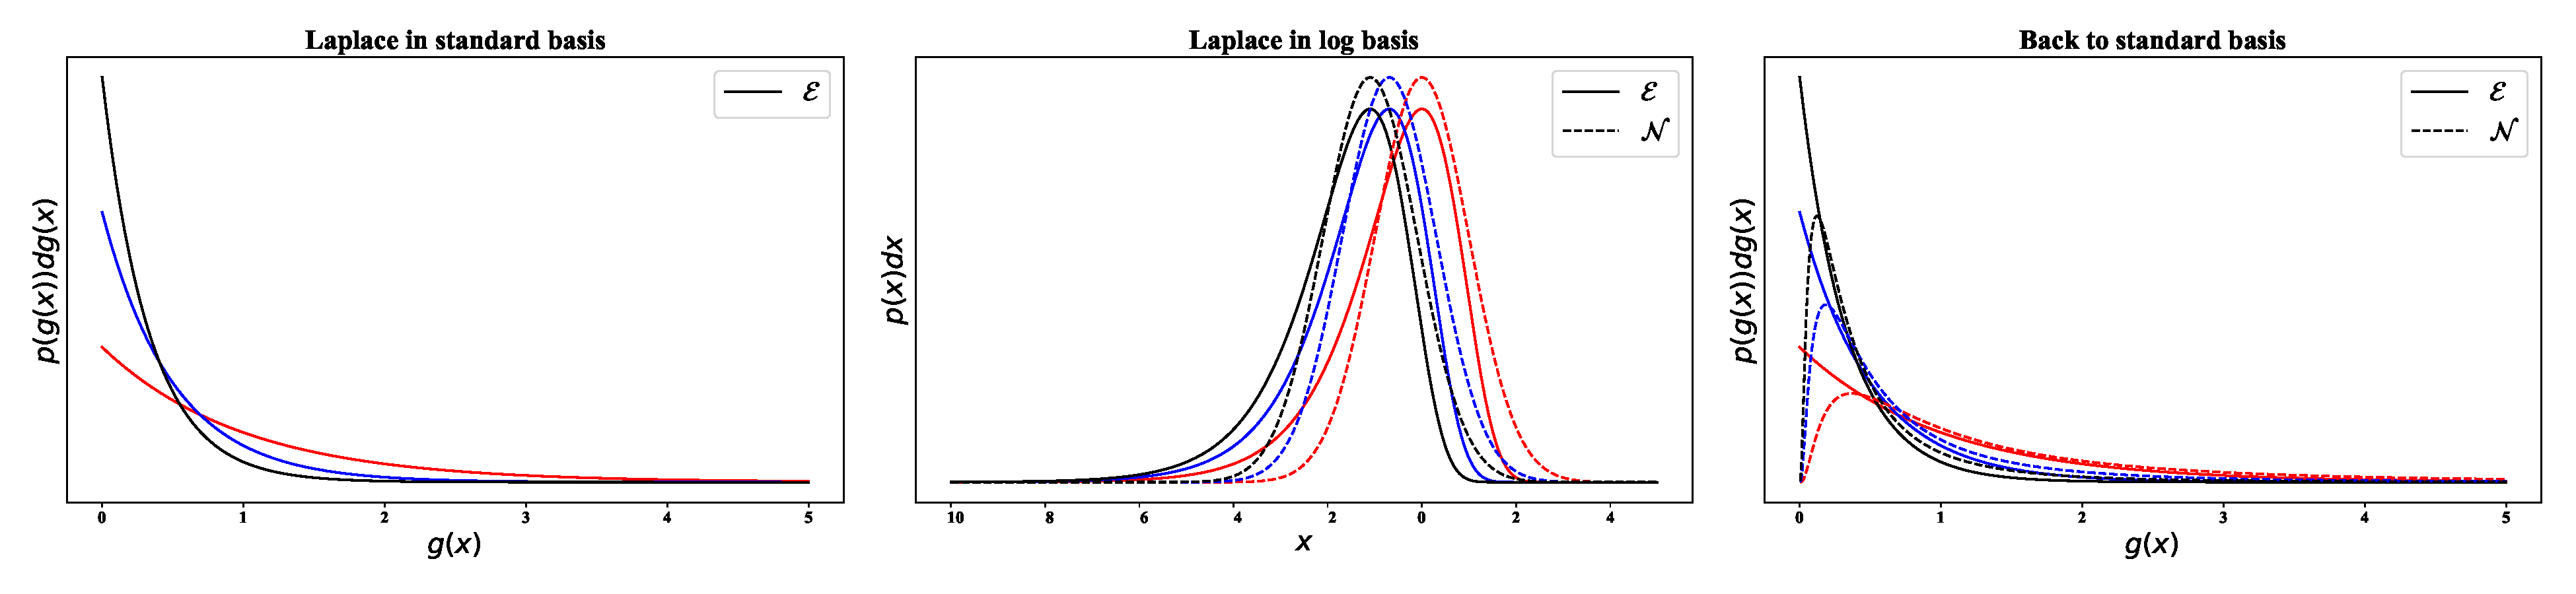
\includegraphics[width=\textwidth]{figures/exponential_log_bridge.pdf}
	\caption{log-Bridge for the Exponential distribution}
	\label{fig:exponential_log_bridge}
\end{figure}

\subsection{Sqrt-transformed Exponential Distribution}

We choose $X = \sqrt{Y}$ and therefore $g(x) = \sqrt{x}$, and $x(y) = g^{-1}(y) = y^2$. Also, $\left\vert \frac{\partial x(y)}{\partial y}\right\vert = 2y$. It follows that the new pdf is 

\begin{subequations}
\begin{align}
\mathcal{E}_{Ysqrt}(y; \lambda) &= \lambda \exp(-\lambda y^2) \cdot 2y \\
&= 2 \cdot \exp\left[\log(y)-\lambda y^2 + \log\lambda\right]
\end{align}
\end{subequations}

with $h(y)=2$, $\phi(y) = (\log(y), y^2))$, $w = (1, -\lambda)$ and $Z(\lambda)=\log\lambda$

\subsubsection{Laplace Approximation of the sqrt-transformed Exponential Distribution}

\begin{align*}
\text{log-pdf: } & \log(2y)-\lambda y^2 + \log\lambda \\
\text{1st derivative: }& \frac{1}{y} - 2\lambda y \\
\text{mode: } & y = \sqrt{\frac{1}{2\lambda}}\\
\text{2nd derivative: }& -\frac{1}{y^2} - 2\lambda\\
\text{insert mode: }& -\frac{1}{\frac{1}{2\lambda}} - 2\lambda = -4\lambda\\
\text{invert \& times -1: }&\sigma^2 = \frac{1}{4\lambda}
\end{align*}

\subsubsection{The Bridge for the sqrt-transformed Exponential Distribution}

\begin{subequations}
\begin{align}
	\mu &= \sqrt{\frac{1}{2\lambda}} \\
	\sigma^2 &= \frac{1}{4\lambda} \\
	\lambda &= \frac{1}{2\mu^2}
\end{align}
\end{subequations}

\begin{figure}[!htb]
	\centering
	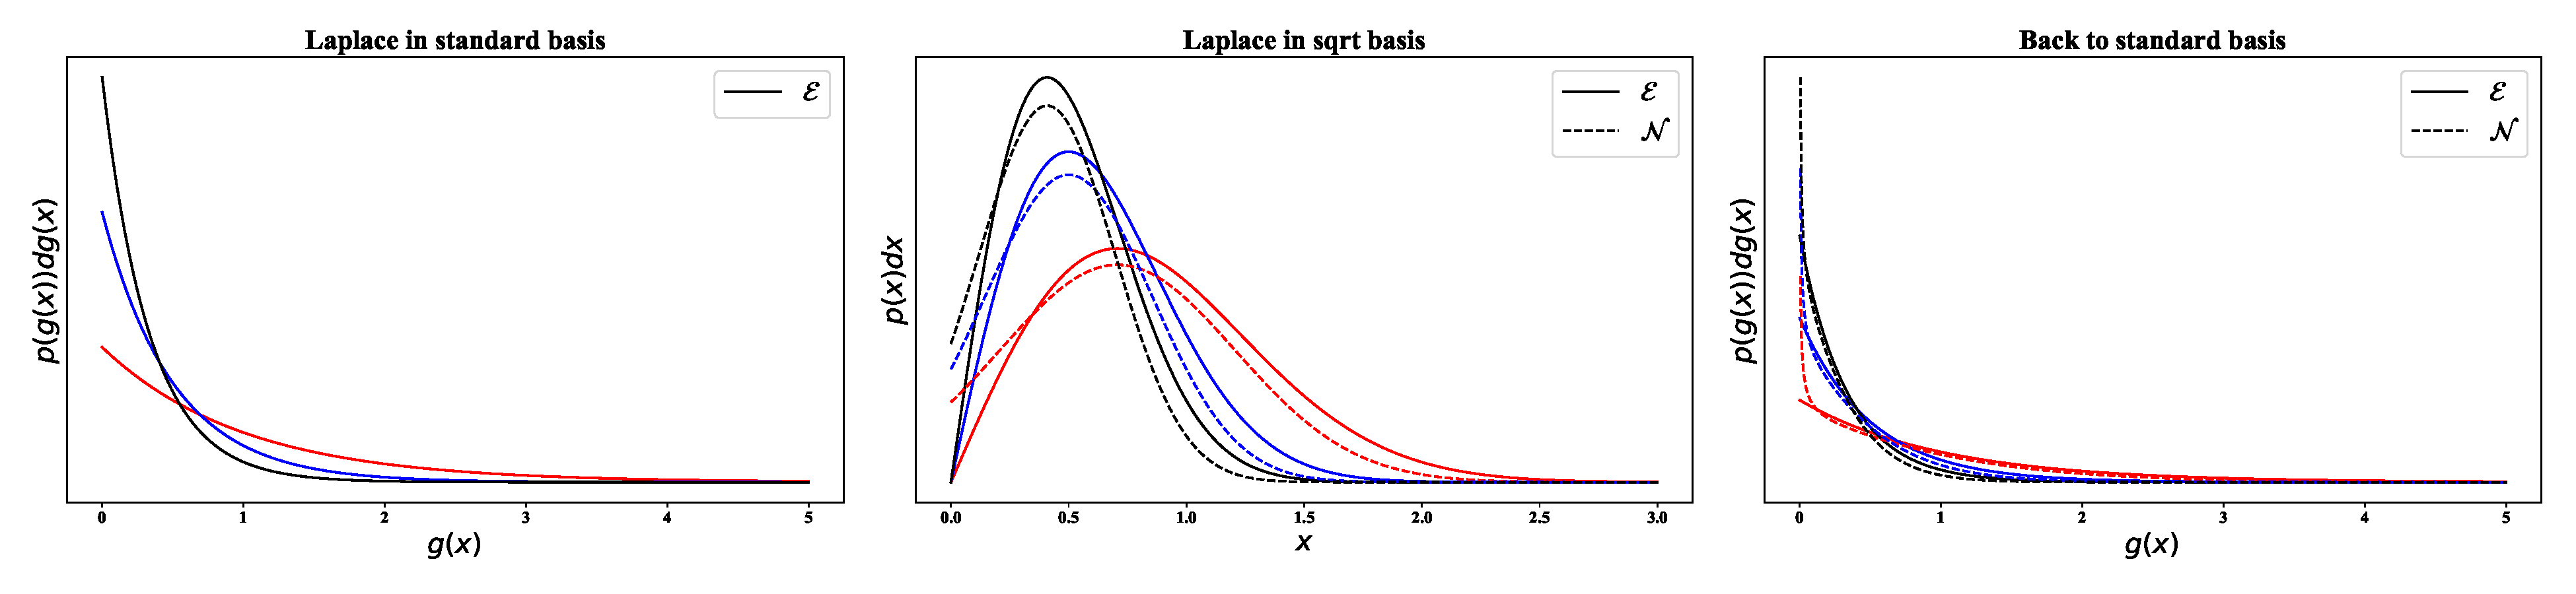
\includegraphics[width=\textwidth]{figures/exponential_sqrt_bridge.pdf}
	\caption{sqrt-Bridge for the Exponential distribution}
	\label{fig:exponential_sqrt_bridge}
\end{figure}

\subsection{Standard Gamma Distribution}

\begin{equation}
	\mathcal{G}_X(x, \alpha, \lambda) = \frac{\lambda^\alpha}{\Gamma(\alpha)} \cdot x^{(\alpha - 1)} \cdot e^{(-\lambda x)}
	\label{eq:gamma_pdf}
\end{equation}

where $\Gamma(\alpha)$ is the Gamma function. This can be written as

\begin{subequations}
\begin{align}
	\mathcal{G}_X(x, \alpha, \lambda) &= \exp \left[(\alpha -1)\log(x) - \lambda x + \alpha \log(\lambda) - \log(\Gamma(\alpha))\right] \\
	&= \frac{1}{x} \exp\left[\alpha\log(x) - \lambda x + \alpha \log(\lambda) - \log(\Gamma(\alpha))\right]
	\label{eq:gamma_exp_family}
\end{align}
\end{subequations}

with $h(x) = \frac{1}{x},\, \phi(x)=(\log x, x),\, w=(\alpha, -\lambda)$ and $Z(\alpha, \lambda) = \log(\Gamma(\alpha)) - \alpha  \log(\lambda)$. 

\subsubsection{Laplace Approximation of the Gamma Distribution}

To get the LPA of the Gamma function in the standard basis we need its mode and the second derivative of the log-pdf. The mode is already known to be $\hat{\theta} = \frac{\alpha -1}{\lambda}$. For the second derivative of the log-pdf we take the log-pdf and derive it twice and insert the mode for $x$:
\begin{align*}
	\text{log-pdf: } &\log\left( \frac{\lambda^\alpha}{\Gamma(\alpha)} \cdot x^{(\alpha - 1)} \cdot e^{(-\lambda x)}\right) \\
	&= \alpha \cdot \log(\lambda) - \log(\Gamma(\alpha)) + (\alpha -1)\log(x) -\lambda x\\
	\text{1st derivative: }& \frac{(\alpha-1)}{x} - \lambda \\
	\text{mode: }&  \frac{(\alpha-1)}{x} - \lambda = 0 \Leftrightarrow x=\frac{\alpha -1}{\lambda}\\
	\text{2nd derivative: }& -\frac{(\alpha-1)}{x^2}\\
	\text{insert mode: }& -\frac{(\alpha-1)}{(\frac{\alpha -1}{\lambda})^2} = -\frac{\lambda^2}{\alpha - 1} \\
	\text{invert and times -1: }&\sigma^2 = \frac{\alpha-1}{\lambda^2}
\end{align*}

The LPA of the Gamma distribution is therefore approximately distributed according to the pdf of $\mathcal{N}(x; \frac{\alpha - 1}{\lambda}, \frac{\alpha-1}{\lambda^2})$.


\subsection{Log-Transform of the Gamma Distribution}

We transform the Gamma Distribution with the Log-Transformation, i.e. $Y = \log(X), g(x) = \log(x), x(y) = g^{-1}(x) = \exp(x)$. Also, $\left\vert \frac{\partial x(y)}{\partial y}\right\vert = \exp(y)$. The transformed pdf is

\begin{subequations}
\begin{align}
\mathcal{G}_{Y\_\log }(y, \alpha, \lambda) &= \frac{\lambda^\alpha}{\Gamma(\alpha)} \cdot x(y)^{(\alpha - 1)} \cdot e^{(-\lambda x(y))} \cdot \exp(y) \\ 
&=\frac{\lambda^\alpha}{\Gamma(\alpha)} \cdot \exp(y)^{\alpha} \cdot e^{(-\lambda \exp(y))} \\
&= \exp\left[\alpha y - \lambda\exp(y) - \Gamma(\alpha) + \alpha\log(\lambda) \right]
\end{align}
\end{subequations}

with exponential family parameters $h(y) = 1$, $\phi(y) = (y, \exp(y)), \eta = (\alpha, -\lambda)$ and $Z(\alpha, \lambda) = \log(\Gamma(\alpha)) - \alpha  \log(\lambda)$. 


\subsubsection{Laplace Approximation of the log-transformed Gamma Distribution}

To get the LPA of the Gamma distribution in the transformed basis we need to calculate its mode and the second derivative of the log-pdf. To get the mode we take the first derivative and set it to zero. 

\begin{align*}
\text{log-pdf: } &= \alpha \log(\lambda) - \log(\Gamma(\alpha)) + \alpha y - \lambda \exp(y)\\
\text{1st derivative: }&  \alpha - \lambda \exp(y)\\
\text{mode: }& \alpha - \lambda \exp(y) = 0 \Leftrightarrow y = \log\left(\frac{\alpha}{\lambda}\right)\\
\text{2nd derivative: }&  -\lambda \exp(y)\\
\text{insert mode: }& -\lambda \exp(\log\left(\frac{\alpha}{\lambda}\right)) = -\alpha \\
\text{invert and times -1: }&\sigma^2 = \frac{1}{\alpha}
\end{align*}

The resulting Guassina is $N(y; \log\left(\frac{\alpha}{\lambda}\right), \frac{1}{\alpha})$.

\subsubsection{The bridge for the log-transformation}

We already know how to get $\mu$ and $\sigma$ from $\lambda$ and $\alpha$. To invert we calculate $\mu = \log(\alpha/\lambda) \Leftrightarrow \lambda= \alpha/\exp(\mu)$ and insert $\alpha=\sigma^2$. In summary we have

\begin{subequations}
\begin{align}
\mu &= \log\left(\frac{\alpha}{\lambda}\right) \\
\sigma^2 &= \frac{1}{\alpha} \\
\lambda &=  \frac{1}{\exp(\mu)\sigma^2}\\
\alpha &= \frac{1}{\sigma^2}
\end{align}
\end{subequations}

\begin{figure}[!htb]
	\centering
	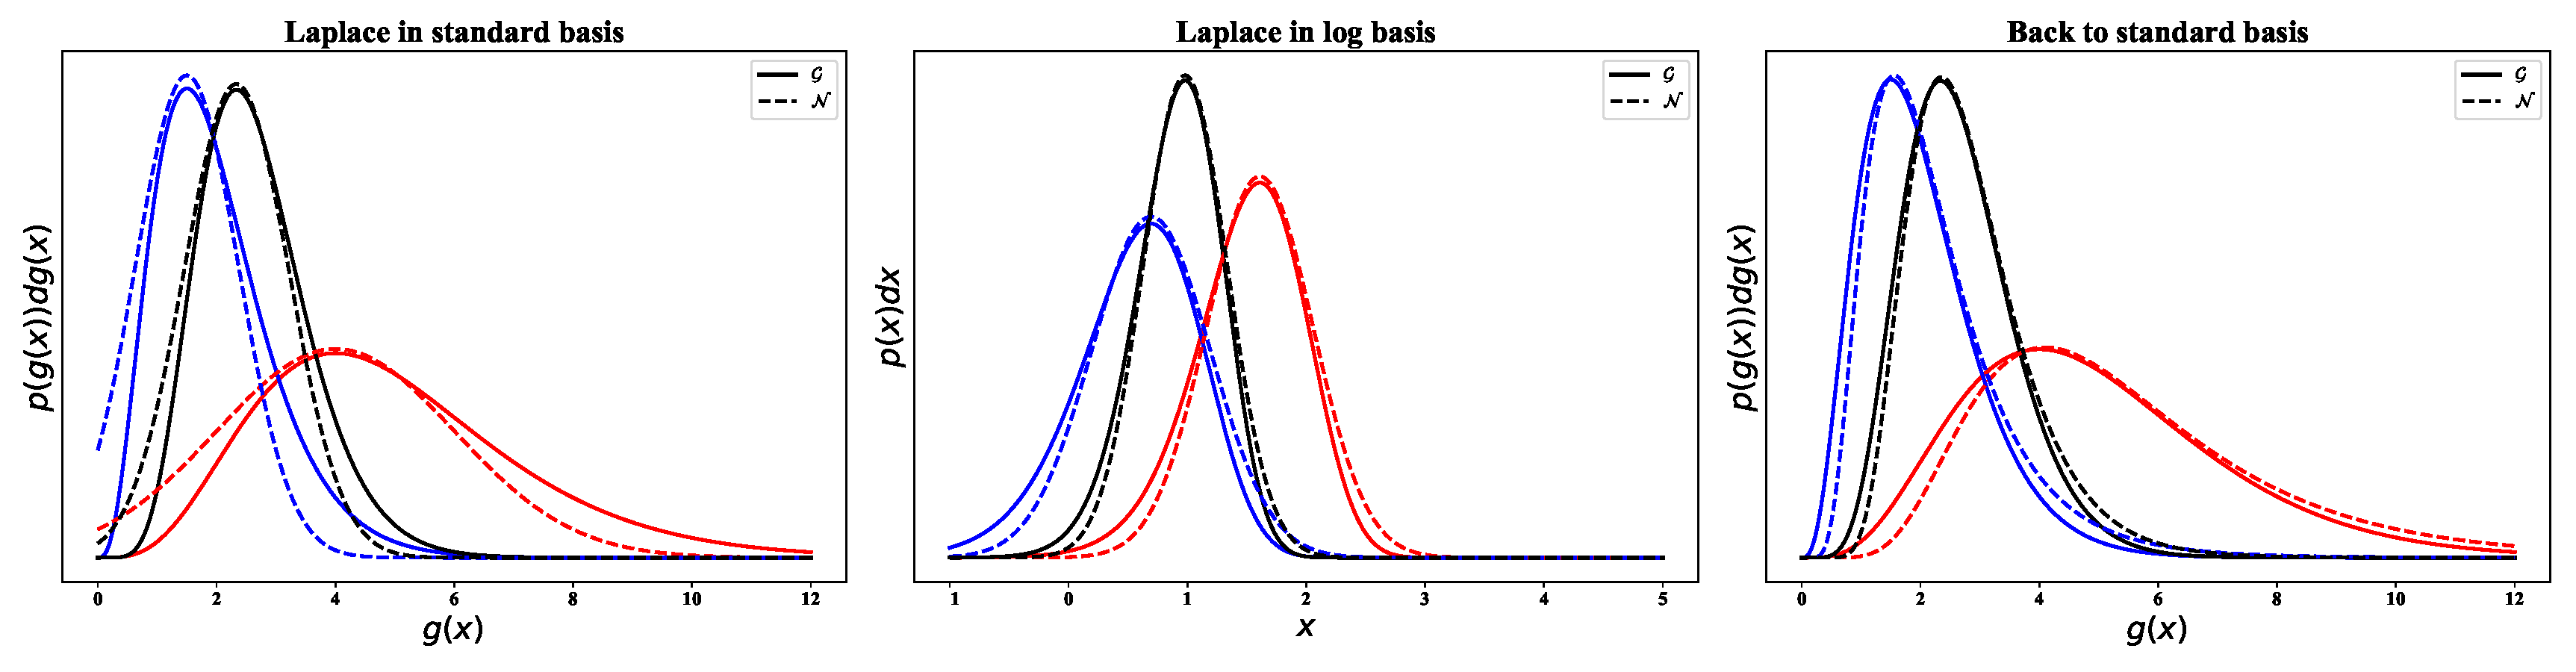
\includegraphics[width=\textwidth]{figures/Gamma_log_bridge.pdf}
	\caption{log-Bridge for Gamma distribution}
	\label{fig:gamma_log_bridge}
\end{figure}

\subsection{Sqrt-Transform of the Gamma Distribution}

\subsubsection{Sqrt-Transformation}

We transform the Gamma Distribution with the sqrt-transformation, i.e. $Y = \sqrt{X}, g(x) = \sqrt{x},x_1(y) =  g_1^{-1}(y) = -y^2, x_2(y) = g_2^{-1}(y) = y^2$ and $\left\vert\frac{\partial x_i(y)}{\partial y} \right\vert = \left\vert\frac{\partial g_i^{-1}(y)}{\partial y} \right\vert = \vert 2y \vert$. We use the same `trick' as in Subsection \ref{subsec:chi2-normal} to split up the transformation in two parts. 

\begin{subequations}
\begin{align}
\mathcal{G}_Y(y) &=  \frac{1}{2} \cdot \mathcal{G}_X(x_1(y)) \left\vert\frac{\partial x_1(y)}{\partial y} \right\vert \mathbf{1}_\wedge(y) +  \frac{1}{2} \cdot\mathcal{G}_X(x_2(y)) \left\vert\frac{\partial x_2(y)}{\partial y} \right\vert \mathbf{1}_\wedge(y) \\
&= \frac{1}{2y^2} \exp[\alpha \log(y^2) - \lambda y^2 - A(\alpha, \lambda)] |2y| \mathbf{1}_{(-\infty, 0)}(y) + \frac{1}{2y^2} \exp[\alpha \log(y^2) - \lambda y^2 - A(\alpha, \lambda)] |2y| \mathbf{1}_{[0, \infty)}(y) \\
&= \frac{1}{\sqrt{y}}\exp[2\alpha \log(y) - \lambda y^2 - A(\alpha, \lambda)] \mathbf{1}_{(-\infty, +\infty)}(y) \\
&= \frac{1}{\sqrt{y}}\exp[2\alpha \log(y) - \lambda y^2 - A(\alpha, \lambda)]
\end{align}
\end{subequations}

which is defined on the entirety of $\mathbb{R}$ and is an exponential family with $h(y) = \frac{1}{\sqrt{y}},\, \phi(y)=(\log(y), y^2), \,w=(2\alpha, -\lambda)$ and $Z(\alpha, \lambda) = \log(\Gamma(\alpha)) - \alpha \log(\lambda)$.

\subsubsection{Laplace Approximation of the sqrt-transformed Gamma Distribution}

To get the LPA of the Gamma distribution in the transformed basis we need to calculate its mode and the second derivative of the log-pdf. To get the mode we take the first derivative and set it to zero. 

\begin{align*}
\text{log-pdf: } &(2\alpha-1) \log(y) - \lambda y^2 + \alpha \log(\lambda) - \log(\Gamma(\alpha)) \\
\text{1st derivative: }&  \frac{2\alpha-1}{y} - 2\lambda y\\
\text{mode: }& \frac{2\alpha-1}{y} - 2\lambda y = 0 \Leftrightarrow y = \sqrt{\frac{\alpha-0.5}{\lambda}}\\
\text{2nd derivative: }&  -\frac{2\alpha-1}{x^2} - 2\lambda\\
\text{insert mode: }& -\frac{2\alpha-1}{\frac{\alpha-0.5}{\lambda}} - 2\lambda = -4\lambda\\
\text{invert and times -1: }& \sigma^2 = \frac{1}{4\lambda}
\end{align*}

Therefore the LPA now is $\mathcal{N}\left(\sqrt{\frac{\alpha-0.5}{\lambda}}, \frac{1}{4\lambda} \right)$.

\subsubsection{The bridge for the sqrt-transformation}

We already know how to get $\mu$ and $\sigma$ from $\lambda$ and $\alpha$. To invert we calculate $\mu = \sqrt{\frac{\alpha-0.5}{\lambda}} \Leftrightarrow \alpha = \frac{\mu^2}{\lambda}-0.5$ and insert $\lambda=\frac{4}{\sigma^2}$. In summary we have

\begin{subequations}
\begin{align}
\mu &= \sqrt{\frac{\alpha-0.5}{\lambda}} \\
\sigma^2 &= \frac{1}{4\lambda} \\
\lambda &= \frac{4}{\sigma^2} \\
\alpha &= \frac{4\mu^2}{\sigma^2}+0.5 
\end{align}
\end{subequations}

\begin{figure}[!htb]
	\centering
	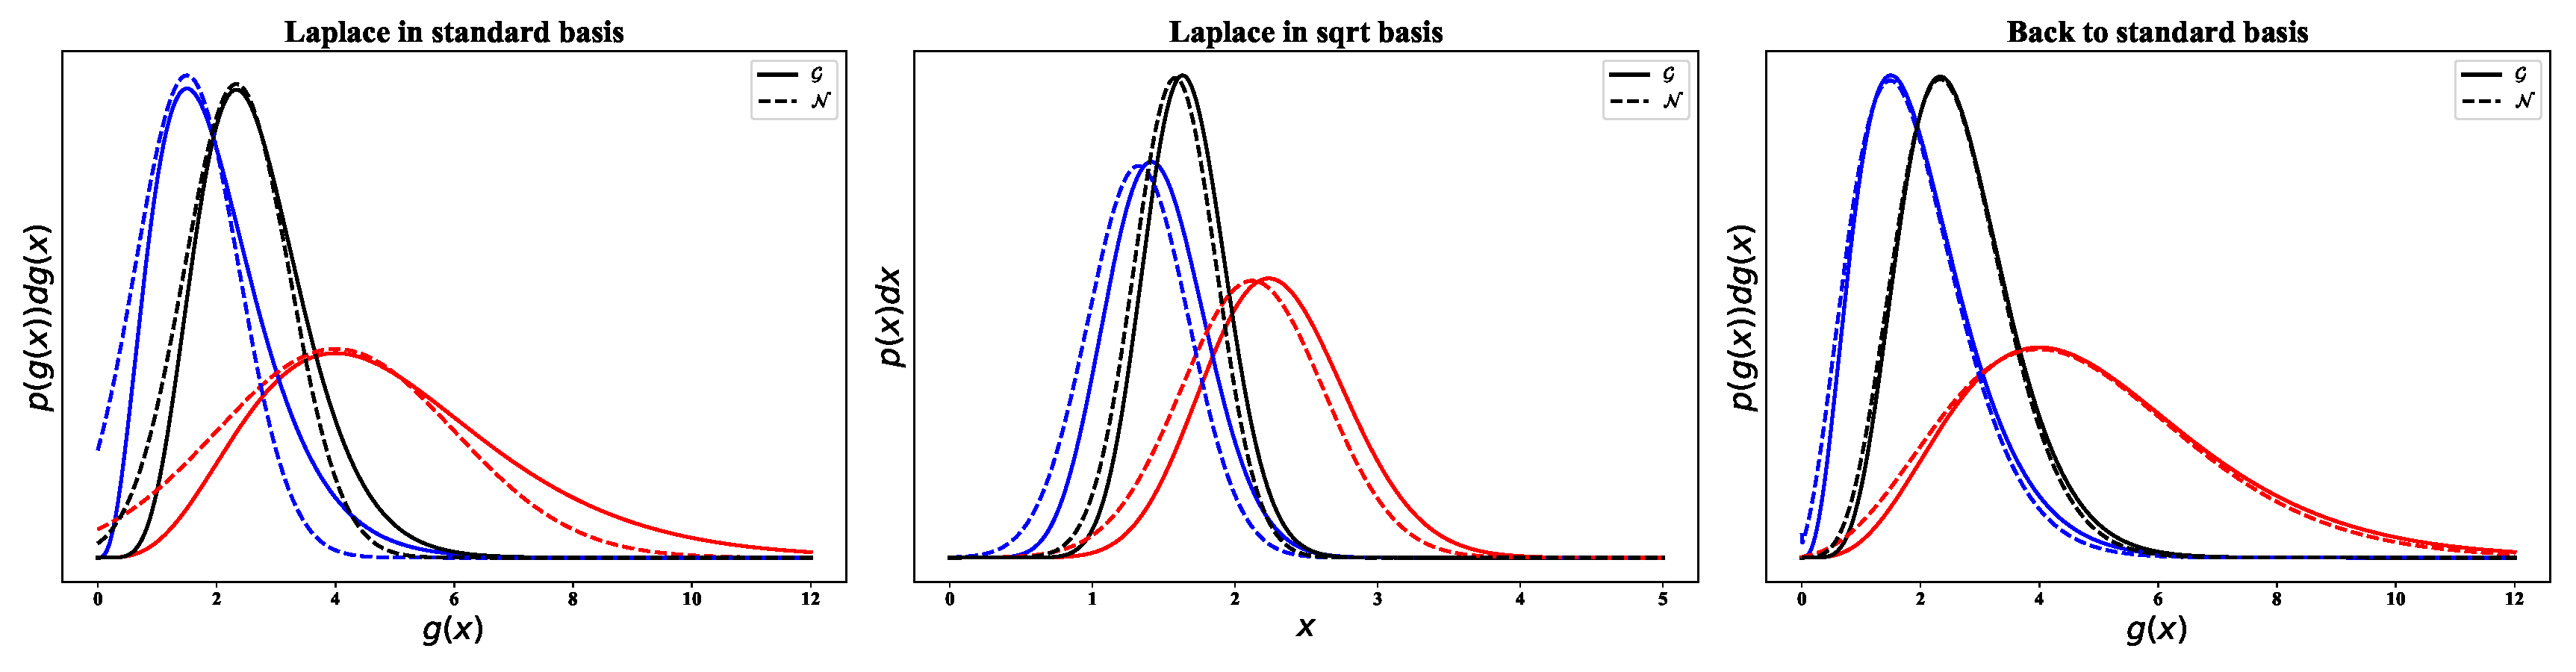
\includegraphics[width=\textwidth]{figures/Gamma_sqrt_bridge.pdf}
	\caption{sqrt-Bridge Gamma}
	\label{fig:gamma_sqrt_bridge}
\end{figure}

\subsection{Standard Inverse Gamma Distribution}

The pdf of the inverse gamma is 

\begin{equation}
	f(x, \alpha, \lambda) = \frac{\lambda^{\alpha}}{\Gamma(\alpha)} x^{-\alpha-1} \exp(-\frac{\lambda}{x})
	\label{eq:pdf_inverse_gamma}
\end{equation}

where $\Gamma$ is the Gamma function. This can be rewritten as

\begin{equation}
	f(x, \alpha, \lambda) = \exp \frac{1}{x}\left[-\alpha\log(x) - \lambda/x + \alpha \log(\lambda) -\log\Gamma(\alpha)\right]
	\label{eq:exp_inverse_gamma}
\end{equation}

where $h(x) = \frac{1}{x}$, $\phi(x)=(\log(x), x), w= (-\alpha, -\lambda)$ and $Z(\alpha,\lambda) = \log\Gamma(\alpha) - \alpha\log\lambda$.

\subsubsection{Laplace Approximation of the standard inverse gamma distribution}

\begin{align*}
\text{log-pdf: } &(-\alpha-1)\log(x) - \lambda/x + \alpha \log(\lambda) -\log\Gamma(\alpha) \\
\text{1st derivative: }&  \frac{-\alpha-1}{x} + \frac{\lambda}{x^2}\\
\text{mode: }& \frac{-\alpha-1}{x} + \frac{\lambda}{x^2} = 0 \Leftrightarrow x = \frac{\lambda}{a+1}\\
\text{2nd derivative: }&  \frac{\alpha+1}{x^2} - 2\frac{\lambda}{x^3}\\
\text{insert mode: }& \frac{\alpha+1}{\frac{\lambda}{a+1}^2} - 2\frac{\lambda}{\frac{\lambda}{a+1}^3} = -\frac{(\alpha +1)^3}{\lambda^2} \\
\text{invert and times -1: }&\sigma^2 = \frac{\lambda^2}{(\alpha +1)^3}
\end{align*}

with $q(x) = \mathcal{N}(x; \mu = \frac{\lambda}{a+1}, \sigma^2 =\frac{\lambda^2}{(\alpha +1)^3} )$. 

\subsection{Log-Transform of the inverse Gamma distribution}

We transform the Inverse Gamma distribution with the log-transformation, i.e. $Y = \log(X)$. Therefore $g(x) = \log(x)$, and thereby $x(y) = g^{-1}(x) = \exp(y)$. It follows that the new pdf is 

\begin{align}
	f_{Y\_\log}(y, \alpha, \lambda) &= \frac{\lambda^{\alpha}}{\Gamma(\alpha)} \exp(y)^{-\alpha-1} \exp(-\lambda/\exp(y)) \cdot \exp(y) \\
	&=  \frac{\lambda^{\alpha}}{\Gamma(\alpha)} \exp(y)^{-\alpha} \exp(-\lambda/\exp(y)) \\
	&= \exp\left[-\alpha x - \frac{\lambda}{\exp(x)} - \log\Gamma(\alpha) + \alpha\log(\lambda)\right]
	\label{eq:inv_gamma_trans_pdf}
\end{align}


with $h(y) = 1, \phi(y) = (y, \exp(y)), w=(-\alpha, \lambda)$ and $Z(\alpha, \lambda) = \log\Gamma(\alpha) - \alpha \log \lambda$.

\subsubsection{Laplace Approximation of the log-transformed Inverse Gamma Distribution}


\begin{align*}
\text{log-pdf: } &-\alpha y - \frac{\lambda}{\exp(y)} + C \\
\text{1st derivative: }&  -\alpha + \frac{\lambda}{\exp(y)}\\
\text{mode: }&  -\alpha + \frac{\lambda}{\exp(y)} = 0 \Leftrightarrow y = \log(\lambda/\alpha)\\
\text{2nd derivative: }&  -\frac{\lambda}{\exp(y)}\\
\text{insert mode: }&  -\frac{\lambda}{\exp(\log(\lambda/\alpha))} = -\alpha\\
\text{invert and times -1: }&\sigma^2 = \frac{1}{\alpha}
\end{align*}

\subsubsection{The Bridge for the log-transformed Inverse Gamma Distribution}

\begin{align}
	\mu &= \log\left(\frac{\lambda}{\alpha}\right) \\
	\sigma^2 &= \frac{1}{\alpha} \\
	\alpha &= \frac{1}{\sigma^2}\\
	\lambda &= \frac{\exp(\mu)}{\sigma^2}\\
\end{align}

\begin{figure}
	\centering
	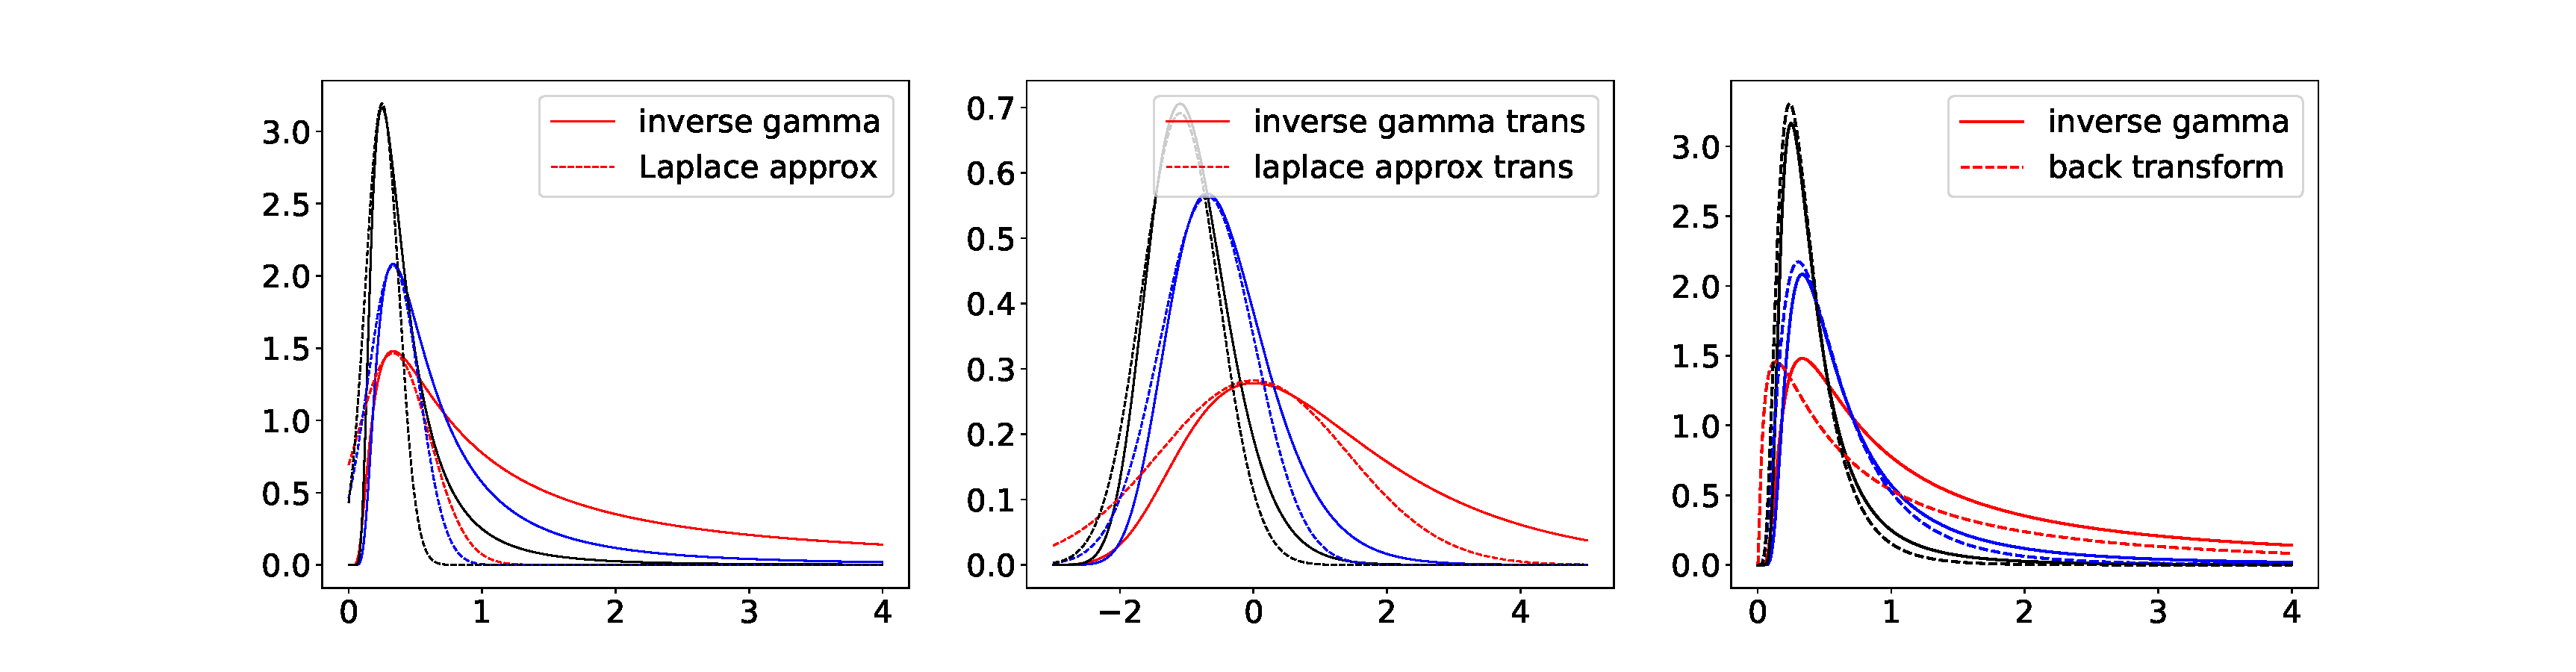
\includegraphics[width=\textwidth]{figures/inverse_gamma_playground.pdf}
	\caption{inverse gamma comparison}
	\label{fig:inverse_gamma_comparison}
\end{figure}

\subsection{Sqrt-Transform of the inverse Gamma distribution}

We transform the Inverse Gamma distribution with the sqrt-transformation, i.e. $Y = \sqrt{X}$. Therefore $g(x) = \sqrt{x}$, and thereby $x(y) = g^{-1}(x) = y^2$. It follows that the new pdf is 

\begin{align}
f_{Y\_\log}(y, \alpha, \lambda) &= \frac{\lambda^{\alpha}}{\Gamma(\alpha)} y^{2(-\alpha-1)} \exp(-\lambda/y^2)) \cdot 2y \\
&=  \frac{\lambda^{\alpha}}{\Gamma(\alpha)} y^{-2\alpha-\frac{1}{2}} \exp(-\lambda/y^2)) \\
&= \frac{1}{\sqrt{y}}\exp\left[-2\alpha \log(y) - \frac{\lambda}{y^2} - \log\Gamma(\alpha) + \alpha\log(\lambda)\right]
\label{eq:inv_gamma_sqrt_pdf}
\end{align}


with $h(y) = \frac{1}{\sqrt{y}}, \phi(y) = (\log(y), y^2), w=(-2\alpha, -\lambda)$ and $Z(\alpha, \lambda) = \log\Gamma(\alpha) - \alpha \log \lambda$.

\subsubsection{Laplace Approximation of the sqrt-transformed Inverse Gamma Distribution}

\begin{align*}
\text{log-pdf: } &(-2\alpha-1)\log(y) - \frac{\lambda}{y^2} + C \\
\text{1st derivative: }& -\frac{2\alpha+1}{y} + 2\frac{\lambda}{y^3} \\
\text{mode: }&  y = \sqrt{\frac{\alpha+0.5}{\lambda}}\\
\text{2nd derivative: }&  \frac{2\alpha+1}{y^2} - 6\frac{\lambda}{y^4}\\
\text{insert mode: }&  -4\frac{(\alpha+0.5)^2}{\lambda}\\
\text{invert and times -1: }&\sigma^2 = \frac{\lambda}{4 (\alpha+0.5)^2}
\end{align*}

yielding $q(y) = \mathcal{N}(y; \mu = \sqrt{\frac{\alpha+0.5}{\lambda}}, \sigma^2 = \frac{\lambda}{4 (\alpha+0.5)^2})$. 

\subsubsection{The Bridge for the sqrt-transformed Inverse Gamma Distribution}

\begin{align}
\mu &= \sqrt\frac{\lambda}{\alpha} \\
\sigma^2 &= \frac{\lambda}{4\alpha^2} \\
\alpha &= \frac{\mu^2}{4\sigma^2}-0.5\\
\lambda &= \frac{\mu^4}{4\sigma^2}\\
\end{align}

TODO:figure

\subsection{Standard Chi-squared distribution}

The pdf of the Chi-squared distribution in the standard basis is

\begin{subequations}
\begin{align}\label{eq:chi2_pdf}
	\chi^2_X(x, k) &= \frac{1}{2^{k/2}\Gamma(k/2)}  x^{k/2 -1} \exp(-x/2) \\
	&= \frac{1}{x}\exp \left[(k/2)\log(x) - x/2 - \log(2^{k/2}\Gamma(k/2))\right]
\end{align} 
\end{subequations}

with $h(x)=\frac{1}{x}$, $\phi(x) = (\log(x), x), w = k/2$ and $Z(k) = \log(2^{k/2}\Gamma(k/2))$.

\subsubsection{Laplace approximation of the standard Chi-squared distribution}

\begin{align*}
\text{log-pdf: } &(k/2-1)\log(x) - x/2 - \log(2^{k/2}\Gamma(k/2)) \\
\text{1st derivative: }&  \frac{k/2-1}{x} - \frac{1}{2} \\
\text{mode: }&  \frac{k/2-1}{x} - \frac{1}{2} = 0 \Leftrightarrow x = k-2\\
\text{2nd derivative: }&  -\frac{k/2-1}{x^2}\\
\text{insert mode: }& -\frac{k/2-1}{(k-2)^2} = -\frac{(k-2)}{2(k-2)^2}\\
\text{invert and times -1: }&\sigma^2 = 2(k-2)
\end{align*}

\subsection{Log-Transformed Chi-squared distribution}

we transform the distribution with $g(x) = \log(x)$, i.e. $x(y) = g^{-1}(x) = \exp(y)$. The new pdf becomes

\begin{subequations}
\begin{align}
	\chi^2_{Y\_\log}(y,k) &= \frac{1}{2^{k/2}\Gamma(k/2)}  \exp(y)^{k/2 -1} \exp(-\exp(y)/2) \cdot \exp(y) \\
	&= \frac{1}{2^{k/2}\Gamma(k/2)}  \exp(y)^{k/2} \exp(-\exp(y)/2) \\
	&= \exp\left[\frac{k}{2}y - \frac{\exp(y)}{2} - \log(2^{k/2}\Gamma(k/2))\right]
\end{align}
\end{subequations}

with $h(y) = 1, \phi(y) =(y, \exp(y)), \eta=(k/2)$ and $Z(k) =  \log(2^{k/2}\Gamma(k/2))$. 

\subsubsection{Laplace approximation of the log-transformed Chi-squared distribution}

\begin{align*}
\text{log-pdf: } &\frac{k}{2}y - \frac{\exp(y)}{2} - \log(2^{k/2}\Gamma(k/2)) \\
\text{1st derivative: }&  \frac{k}{2} - \frac{\exp(y)}{2} \\
\text{mode: }& k/2 - \frac{\exp(y)}{2} = 0 \Leftrightarrow y = \log(k)\\
\text{2nd derivative: }&  -\frac{\exp(y)}{2}\\
\text{insert mode: }& -\frac{\exp(y)}{2} = -k/2\\
\text{invert and times -1: }&\sigma^2 = 2/k
\end{align*}

which yields the Laplace Approximation $q(y) = \mathcal{N}(y; \mu= \log(k), \sigma^2 = 2/k)$.

\subsubsection{The Bridge for log-transform}

\begin{subequations}
\begin{align}
	\mu &= \log(k) \\
	\sigma^2 &= 2/k \\
	k &= \exp(\mu) \\
	k &= 2/\sigma^2
\end{align}
\end{subequations}

\begin{figure}[!htb]
	\centering
	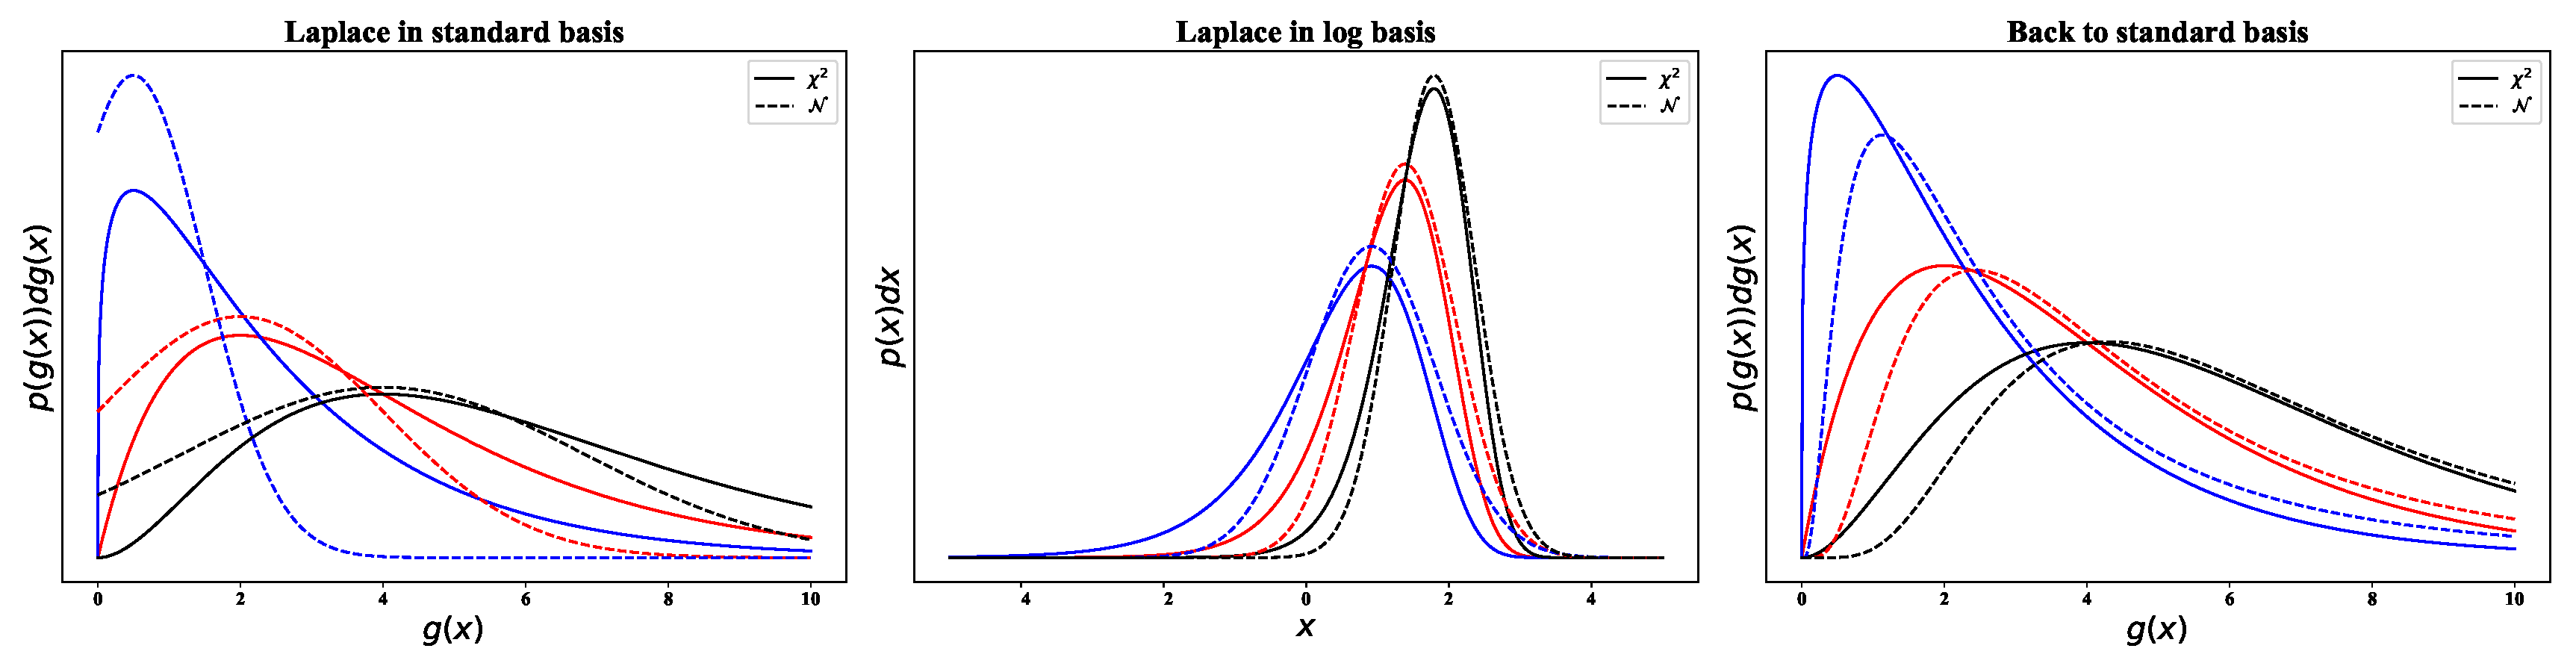
\includegraphics[width=\textwidth]{figures/chi2_log_bridge.pdf}
	\caption{Chi-squared log bridge}
	\label{fig:chi2_log_bridge}
\end{figure}

\subsection{Sqrt-Transformed Chi-squared distribution}

we transform the distribution with $g(x) = \sqrt{x}$, i.e. $x(y) = g^{-1}(x) = y^2$. The new pdf becomes

\begin{subequations}
\begin{align}
\chi^2_{Y_sqrt}(y,k) &= \frac{1}{2^{k/2}\Gamma(k/2)}  y^{2(k/2 -1)} \exp(-y^2/2) \cdot 2y \\
		 &= \frac{1}{2^{k/2}\Gamma(k/2)}  y^{k} \exp(-\frac{y^2}{2}) \\
		 &= \exp \left[k\log(y) - \frac{y^2}{2} - \log(2^{k/2}\Gamma(k/2))\right]
\end{align}
\end{subequations}

with $h(y) = 1, \phi(y)=(\log(y), y^2), w=(k, 1/2)$ and $Z(k) =  \log(2^{k/2}\Gamma(k/2))$. Note that we drop a factor of 2 because of the explanation given in Section \ref{sec:appendix_A}.

\subsubsection{Laplace approximation of the sqrt-transformed Chi-squared distribution}

\begin{align*}
\text{log-pdf: } &(k\log(y) - \frac{y^2}{2} - \log(2^{k/2}\Gamma(k/2)) \\
\text{1st derivative: }&  \frac{k}{x} -y \\
\text{mode: }& \frac{k}{x} -y = 0 \Leftrightarrow y = \sqrt{k}\\
\text{2nd derivative: }&  -\frac{k}{y^2} - 1\\
\text{insert mode: }& -\frac{k}{k}-1 = -2\\
\text{invert and times -1: }&\sigma^2 = 1/2
\end{align*}

\subsubsection{The Bridge for sqrt-transform}

\begin{subequations}
\begin{align}
\mu &= \sqrt{k} \\
\sigma^2 &= 1/2 \\
k &= \mu^2
\end{align}
\end{subequations}

\begin{figure}[!htb]
	\centering
	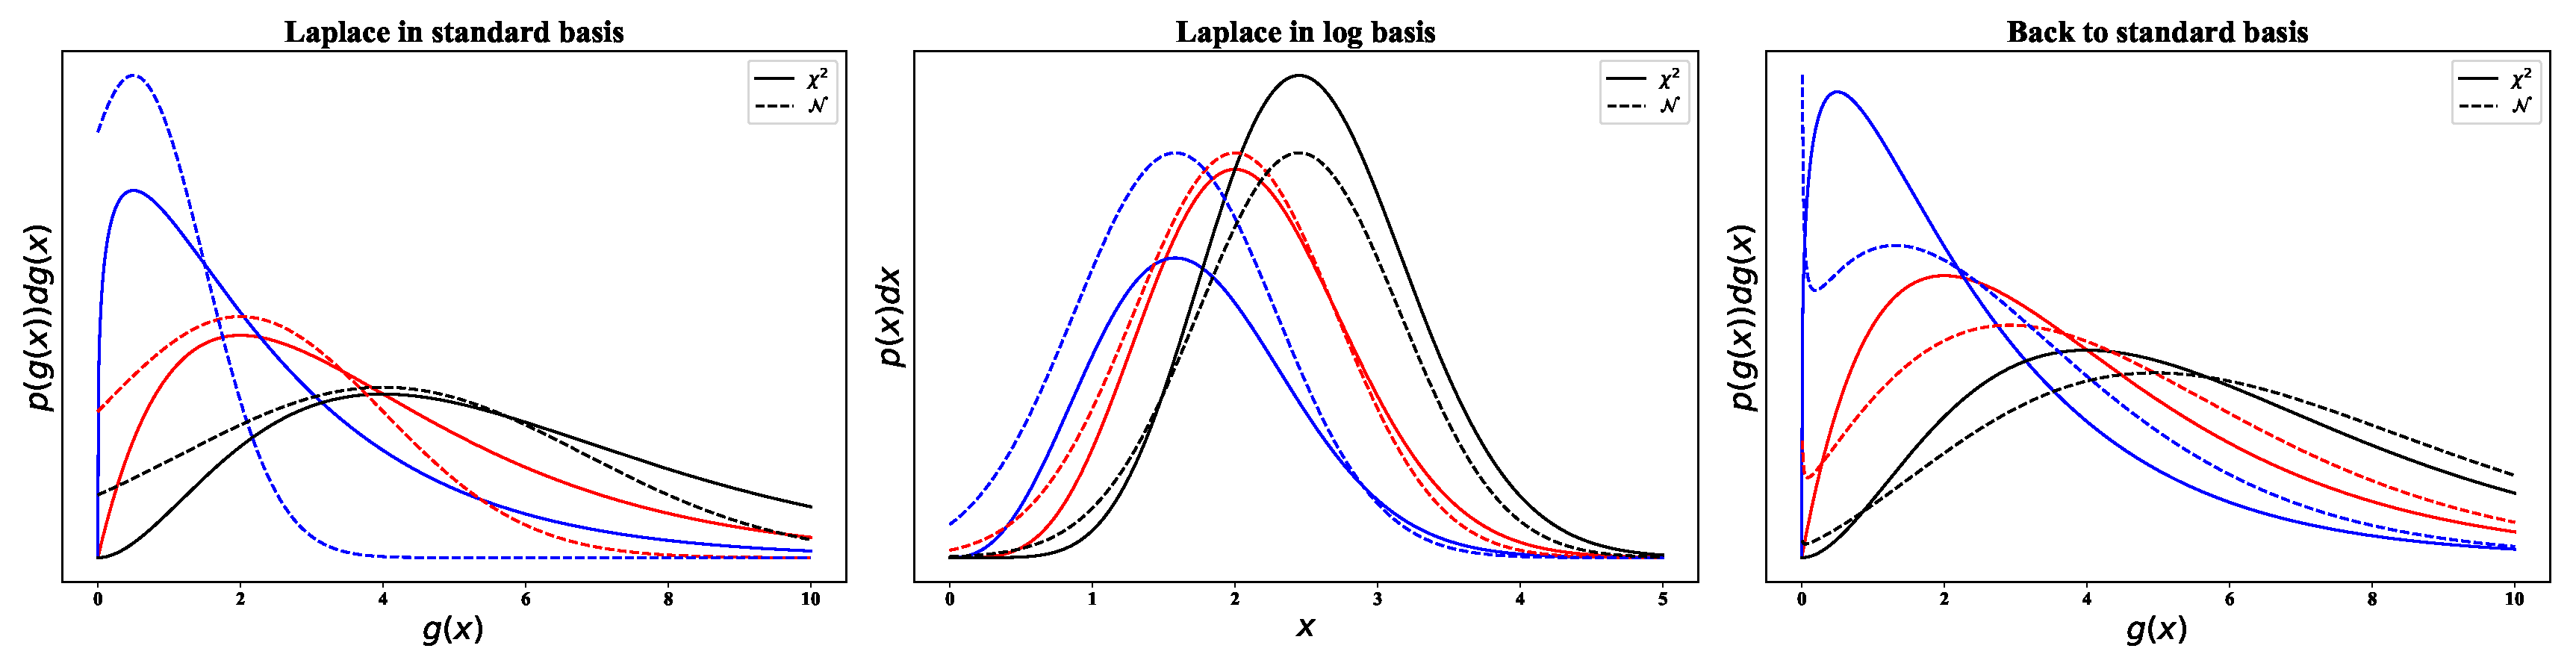
\includegraphics[width=\textwidth]{figures/chi2_sqrt_bridge.pdf}
	\caption{Chi-squared sqrt-bridge}
	\label{fig:chi2_sqrt_bridge}
\end{figure}

\section{Beta Distribution}

\subsection{Standard Beta Distribution}

The pdf of the Beta distribution in the standard basis is

\begin{equation}
	f(x, \alpha, \beta) = \frac{x^{(\alpha - 1)} \cdot (1-x)^{(\beta-1)}}{B(\alpha, \beta)} \\
\end{equation}

where $B(\alpha, \beta) = \frac{\Gamma(\alpha)\Gamma(\beta)}{\Gamma(\alpha + \beta)}$ and $\Gamma(x)$ is the Gamma function.. This can be written as 

\begin{equation}
	f(x, \alpha, \beta) =  \exp\left[(\alpha-1) \log(x) + (\beta-1)\log(1-x) - \log(B(\alpha,\beta)))\right]\\
\end{equation}

With $T=(\log(x), \log(1-x), \eta = (\alpha, \beta)$ and $A(\alpha, \beta) = \log(B(\alpha,\beta)))$. 


\subsubsection{Laplace approximation of the standard Beta distribution}

To get the Laplace approximation we need the mode and Hessian. To get the mode we use the first derivative of the log-pdf and set it to zero. To get the Covariance we use the Hessian at the mode, multiply it with -1 and invert it. 

%The first derivative of the log-pdf is
%
%\begin{equation}
%	\frac{\partial \log(f(x))}{\partial x} = \frac{(\alpha-1)}{x} - \frac{(\beta-1)}{1-x} 
%\end{equation}
%
%To get the mode we set equal to zero and solve for $x$:
%
%\begin{align*}
%	\frac{(\alpha-1)}{x} - \frac{(\beta-1)}{1-x} &= 0  \\
%	\Leftrightarrow \frac{(\alpha-1)}{x} = \frac{(\beta-1)}{1-x}  \\
%	
%\end{align*}

\begin{align*}
\text{log-pdf: } &\log\left( \frac{x^{(\alpha - 1)} \cdot (1-x)^{(\beta-1)}}{B(\alpha, \beta)} \right) \\
&= (\alpha-1) \log(x) + (\beta-1)\log(1-x) - \log(B(\alpha,\beta)))\\
\text{1st derivative: }& \frac{(\alpha-1)}{x} - \frac{(\beta-1)}{1-x}  \\
\text{mode: }& \frac{(\alpha-1)}{x} - \frac{(\beta-1)}{1-x}  = 0 \Leftrightarrow x = \frac{\alpha-1}{\alpha + \beta - 2} \\
\text{2nd derivative: }& \frac{\alpha -1}{x^2} + \frac{\beta - 1}{(1 - x)^2} \\
\text{insert mode: }& \frac{\alpha -1}{\frac{\alpha-1}{\alpha + \beta - 2}^2} + \frac{\beta - 1}{(1 - \frac{\alpha-1}{\alpha + \beta - 2})^2} = \frac{(\alpha + \beta - 2)^3}{(\alpha-1)(\beta-1)}\\
\text{invert: }& \frac{(\alpha -1)(\beta-1)}{(\alpha + \beta - 2)^3}
\end{align*}

The Beta distribution in standard basis is therefore approximated by $N(\mu = \frac{\alpha-1}{\alpha + \beta - 2}, \sigma^2 = \frac{(\alpha -1)(\beta-1)}{(\alpha + \beta - 2)^3})$.

\subsection{Logit-Transform of the Beta distribution}

We transform the Beta distribution using $g(x) = \log(\frac{x}{1-x})$. Therefore $g^{-1}(x) = \sigma(x) = \frac{1}{1+ \exp(-x)}$. This yields the following pdf

\begin{align}
	f_t(x, \alpha, \beta) &= \frac{\sigma(x)^{(\alpha - 1)} \cdot (1 - \sigma(x)^{(\beta -1)})}{B(\alpha, \beta)} \cdot (\sigma(x)(1-\sigma(x)) \\
	&=  \frac{\sigma(x)^{\alpha} \cdot (1 - \sigma(x)^{\beta})}{B(\alpha, \beta)} \nonumber
	\label{eq:beta_logit_trans_pdf}
\end{align}

which can be rewritten to get

\begin{align}
	f_t(x, \alpha, \beta) &= \exp\left[\alpha \log(\sigma(x)) + \beta \log(1-\sigma(x)) - \log B(\alpha, \beta)\right] \\
	&= \exp\left[\alpha \log(\sigma(x)) + \beta \log(\sigma(-x)) - \log B(\alpha, \beta)\right] \\
	&= \exp\left[\alpha \log\left(\frac{1}{1 + \exp(-x)}\right) + \beta \log\left(\frac{1}{1+\exp(x)}\right) - \log B(\alpha, \beta)\right] \\
\end{align}

TODO: THIS FEELS LIKE IT COULD BE SIMPLIFIED BUT I CANNOT FIND THE SOLUTION

\subsubsection{Laplace approximation of the logit transformed Beta distribution}

mode and variance of log pdf blablabla

\begin{align*}
\text{log-pdf: } &\log\left( \frac{\sigma(x)^{\alpha} \cdot (1 - \sigma(x)^{\beta})}{B(\alpha, \beta)} \right) \\
&= \alpha \log(\sigma(x)) + \beta \log(1 - \sigma(x)) - \log(B(\alpha, \beta))\\
\text{1st derivative: }&  \alpha (1 - \sigma(x)) - \beta \sigma(x)\\
\text{mode: }& \alpha (1 - \sigma(x)) - \beta \sigma(x) = 0 \Leftrightarrow x = -\log(\frac{\beta}{\alpha}) \\
\text{2nd derivative: }& (\alpha + \beta)\sigma(x)(1 - \sigma(x))  \\
\text{insert mode: }& (\alpha + \beta)\sigma(-\log(\frac{\beta}{\alpha}))(1 - \sigma(-\log(\frac{\beta}{\alpha}))) = \frac{\alpha\beta}{\alpha + \beta}  \\
\text{invert: }& \frac{\alpha + \beta}{\alpha \beta}
\end{align*}


The LPA is therefore $\mathcal{N}(\mu=-\log(\frac{\beta}{\alpha}), \sigma^2 = \frac{\alpha + \beta}{\alpha \beta})$.

\subsubsection{The Bridge for the logit transformation}


\begin{figure}[!htb]
	\centering
	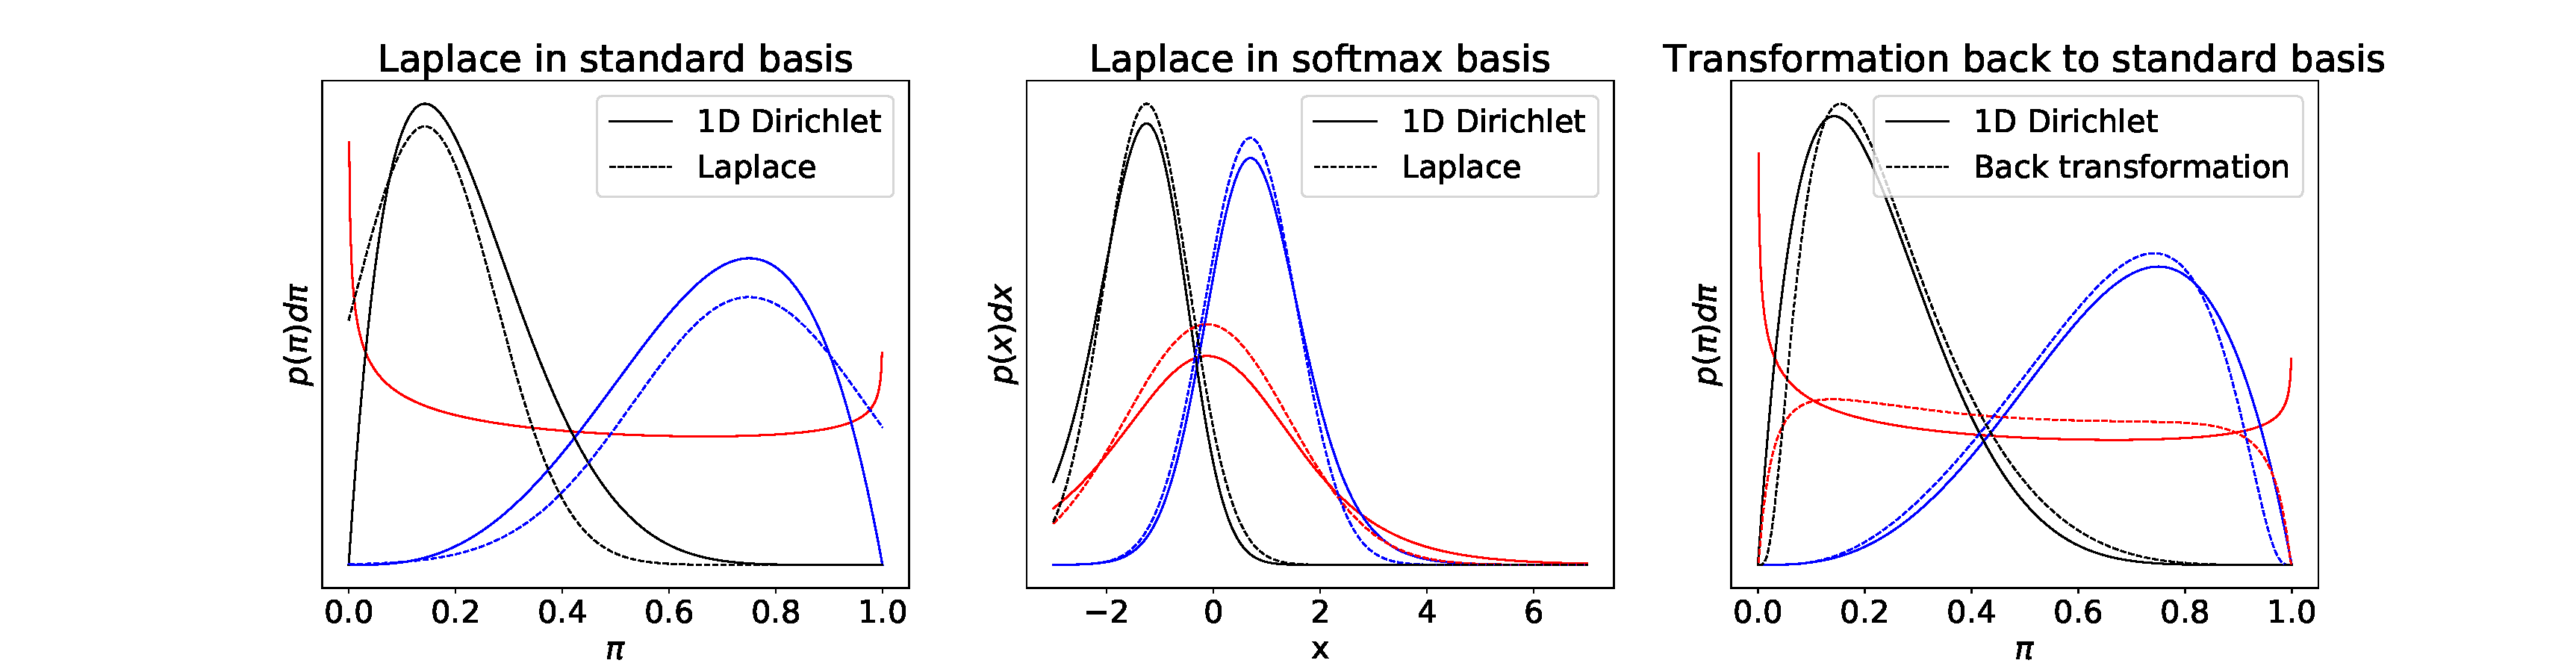
\includegraphics[width=\textwidth]{figures/beta_playground.pdf}
	\caption{beta comparison}
	\label{fig:beta_comparison}
\end{figure}

\section{Dirichlet Distribution}

TODO:REDO THE BRIDGE IN THE EXPONENTIAL FAMILY SETTING. I thought I had already done that but I did not. 

%\begin{figure}[!htb]
%	\centering
%	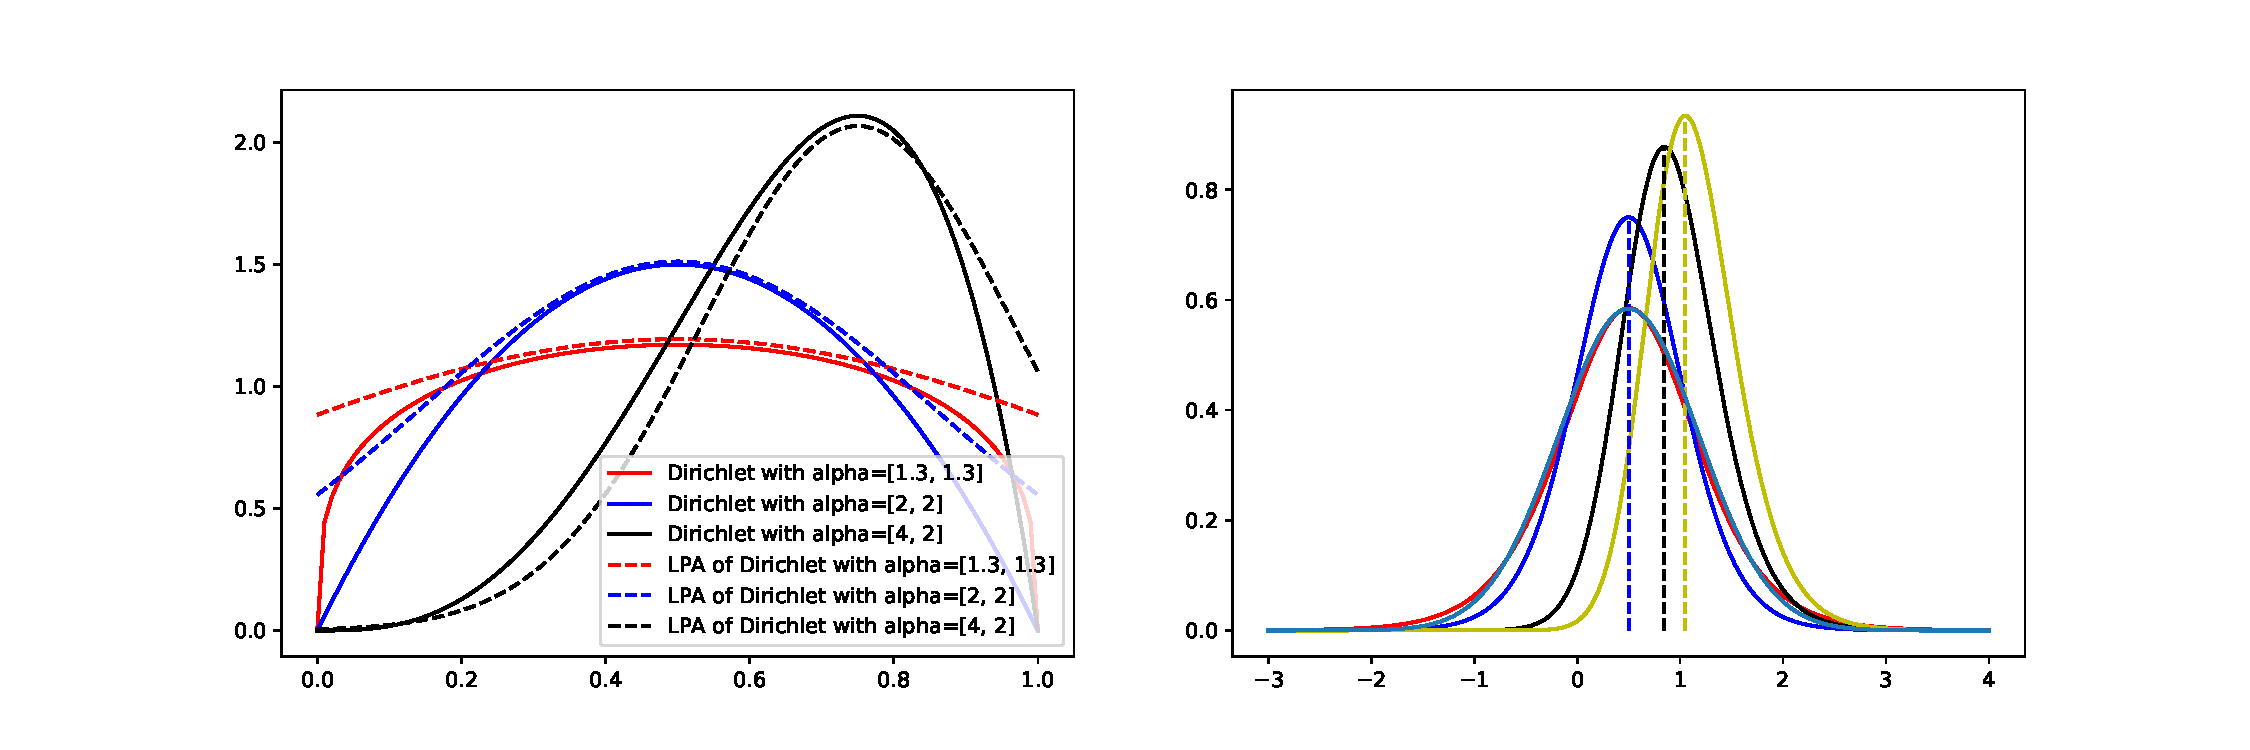
\includegraphics[width=\textwidth]{dirichlet_playground.pdf}
%	\caption{Dirichlet comparison}
%	\label{fig:Dirichlet_comparison}
%\end{figure}


\section{Wishart Distribution}

\subsection{Interlude: Box-product and Kronecker-product}

Kronecker-product: $A \otimes B \in \mathbb{R}^{(m_1m_2) \times (n_1n_2)}$ is defined by $(A \otimes B)_{(i - 1)m_2+j,(k - 1)n_2+l} = a_{il}b_{jk} = (A \otimes B)_{(ij)(kl)}$.

Box-product: $A \boxtimes B \in \mathbb{R}^{(m_1m_2) \times (n_1n_2)}$ is defined by $(A \boxtimes B)_{(i - 1)m_2+j,(k - 1)n_1+l} = a_{ik}b_{jl} = (A \boxtimes B)_{(ij)(kl)}$.

I found this box-product only in two sources, one of which is this: \url{https://researcher.watson.ibm.com/researcher/files/us-pederao/ADTalk.pdf} but it generally seems to be very helpful for matrix derivations with transposed matrices.

\subsection{Standard Wishart distribution}

the pdf of the Wishart is

\begin{equation}
f(X; n,p,V) = \frac{1}{2^{np/2} \left|{\mathbf V}\right|^{n/2} \Gamma_p\left(\frac {n}{2}\right ) }{\left|\mathbf{X}\right|}^{(n-p-1)/2} e^{-(1/2)\operatorname{tr}({\mathbf V}^{-1}\mathbf{X})}
\label{eq:wishart_pdf}
\end{equation}

which can be written as

\begin{equation}
f(X; n,p,V) = \exp \left[(n-p-1)/2 \log(|X|) -(1/2)\operatorname{tr}({\mathbf V}^{-1}\mathbf{X}) - \log\left(2^{np/2} \left|{\mathbf V}\right|^{n/2} \Gamma_p\left(\frac {n}{2}\right )\right) \right]
\end{equation}

with $T=(\log(X), X), \eta=((n-p-1)/2, V^{-1})$ and $A(n,p,V)=\log\left(2^{np/2} \left|{\mathbf V}\right|^{n/2} \Gamma_p\left(\frac {n}{2}\right )\right)$

\subsubsection{Laplace Approximation of the standard Wishart distribution}

Using $\frac{\partial \det(X)}{\partial X} = \det(X)(X^{-1})^\top$ and $\frac{\partial}{\partial X} Tr(AX^\top) = A$ we can calculate the mode by setting the first derivative of the log-pdf to zero

\begin{align*}
\frac{\partial \log f(X; n,p,V)}{\partial X} &= \frac{(n-p-1)\det(X)(X^{-\top})}{2\det(X)} - \frac{V^{-1}}{2} \\
\Rightarrow 0 &= \frac{(n-p-1)X^{-1}}{2} - \frac{V^{-1}}{2} \\
\Leftrightarrow  \frac{(n-p-1)X^{-1}}{2} &= \frac{V^{-1}}{2} \\
\Leftrightarrow X &= (n-p-1)V
\end{align*}

Using the fact that $\frac{\partial X^{-T}}{\partial X} = X^{-T} \boxtimes X^{-1}$ where $\boxtimes$ is the Box-product we compute the second derivative as

\begin{align*}
\frac{\partial^2 \log f(X; n,p,V)}{\partial^2 X} &= -\frac{(n-p-1)}{2} X^{-\top} \boxtimes X^{-1}
\end{align*}

Using $(\alpha A)^{-1} = \alpha^{-1}A^{-1}$, the linearity of the Kronecker product to pull out scalars and $X^{-1} \boxtimes X^{-1} = (X \boxtimes X)^{-1}$ to insert the mode and invert we get:

\begin{align*}
-\frac{(n-p-1)}{2} X^{-1} \boxtimes X^{-1} &= -\frac{(n-p-1)}{2} \frac{1}{(n-p-1)} V^{-1} \otimes \frac{1}{(n-p-1)} V^{-1} \\
&= -\frac{1}{2(n-p-1)}(V \boxtimes V)^{-1} \\
\Rightarrow \Sigma &= 2(n-p-1)(V \boxtimes V)
\end{align*}

In summary, the Laplace approximation of a Wishart distribution in the standard basis is $\mathcal{N}\left(X; (n-p-1)V, 2(n-p-1)(V \boxtimes V)\right)$, where the representation of the symmetric positive definite matrices has been changed from $\mathbb{R}^{n\times n}$ to $\mathbb{R}^{n^2}$.

\subsection{Logm-Transformed Wishart distribution}

we transform the distribution with $g(X) = \text{logm}(X)$, i.e. $g^{-1}(X) = \text{expm}(X)$, where $\text{expm}(X)$ is the matrix exponential and $\text{logm}(X)$ is the matrix logarithm of $X$. The new pdf becomes

\begin{align*}
f(X; n, p, V) &= \frac{1}{2^{np/2} \left|{\mathbf V}\right|^{n/2} \Gamma_p\left(\frac {n}{2}\right ) }{\left|\mathbf{\operatorname{expm}X}\right|}^{(n-p-1)/2} e^{-(1/2)\operatorname{tr}({\mathbf V}^{-1}\mathbf{\operatorname{expm}X})} \cdot |\operatorname{expm}X| \\ 
&= \frac{1}{2^{np/2} \left|{\mathbf V}\right|^{n/2} \Gamma_p\left(\frac {n}{2}\right ) }{\left|\mathbf{\operatorname{expm}X}\right|}^{(n-p+1)/2} e^{-(1/2)\operatorname{tr}({\mathbf V}^{-1}\mathbf{\operatorname{expm}X})} \\ 
&= \exp \left[C + \frac{(n-p+1)}{2} \log(\left|\mathbf{\operatorname{expm}X}\right|)  - \frac{1}{2}\operatorname{tr}({\mathbf V}^{-1}\mathbf{\operatorname{expm}X}) \right]
\end{align*}

with blablabla as expfam values. 

\subsubsection{Laplace Approximation of the logm-transformed Wishart distribution}

To compute the first derivative we use the following

\begin{align}
	\frac{\partial \log(\det(\operatorname{expm}(X)))}{\partial X} 
	&= \frac{\partial \log(\det(\operatorname{expm}(X)))}{\partial \det(\operatorname{expm}(X))} \cdot \frac{\partial \det(\operatorname{expm}(X))}{\partial \operatorname{expm}(X)} \cdot \frac{\partial \operatorname{expm}(X)}{\partial X} \\
	&= \frac{1}{\det(\operatorname{expm}(X))} \cdot \det(\operatorname{expm}(X)) \operatorname{expm}(X)^{-\top} \cdot \operatorname{expm}(X) \\
	&= I_p
\end{align}

where $I_p$ is the identity matrix of size $p$ and we use the fact that the matrix logaritm of a symmetric matrix is symmetric, implying $\operatorname{expm}(X)^{-\top} = \operatorname{expm}(X)^{-1}$. With this we get the 

\begin{align}
	\frac{\partial \log W_{log}}{\partial X} &= \frac{\partial}{\partial X} \left[C + \frac{(n-p+1)}{2} \log(\left|\mathbf{\operatorname{expm}X}\right|)  - \frac{1}{2}\operatorname{tr}({\mathbf V}^{-1}\mathbf{\operatorname{expm}X}) \right] \\
	&=  \frac{(n-p+1)}{2} I_p - \frac{1}{2}V^{-1}\mathbf{\operatorname{expm}X} 
\end{align}

By setting this to zero we get a mode of

\begin{align}
	0 &=  \frac{(n-p+1)}{2} I_p - \frac{1}{2}V^{-1}\mathbf{\operatorname{expm}X} \\
	\Leftrightarrow (n-p+1)I_p &= V^{-1}\mathbf{\operatorname{expm}X} \\
	\Leftrightarrow X &= \operatorname{logm}((n-p+1)V)
\end{align}

For the second derivative we use the fact that

\begin{align}
	\frac{\partial (B\operatorname{expm}(X))_{kl}}{\partial X_{ij}} &= ... \\
	\Leftrightarrow \frac{\partial B\operatorname{expm}(X)}{\partial X} &= \left(B\operatorname{expm}(X) \otimes I_p\right)
\end{align}

yielding

\begin{align}
	\frac{\partial^2 \log W_{log}}{\partial^2 X} &= \frac{\partial \log W_{log}}{\partial X}  \frac{(n-p+1)}{2} I_p - \frac{1}{2}V^{-1}\mathbf{\operatorname{expm}X} \\
	&= -\frac{1}{2}(V^{-1}\mathbf{\operatorname{expm}X} \otimes I_p) \\
	&\overset{\text{mode}}{\Rightarrow} -\frac{1}{2}((n-p+1)V^{-1}V \otimes I_p) \\
	&= -\frac{(n-p+1)}{2} (I_p \otimes I_p)\\
	\Leftrightarrow \Sigma &= \frac{2}{n-p+1} I_{p^2}
\end{align}

where $I_{p^2}$ is an Identity matrix of size $p^2$. 

\subsubsection{The Bridge for logm-tranform}

$\mu$ and $\Sigma$ are already given by the Laplace approximation. Inverting the mode yields an estimate for $V$. 
\begin{align}
	\mu &= \operatorname{logm}((n-p+1)V) \Leftrightarrow \operatorname{expm}(\mu) = (n-p+1)V \Leftrightarrow V = \frac{\operatorname{expm}(\mu)}{(n-p+1)}
\end{align}

where $\mu$ and $V$ are reshaped to a matrix of size $p\times p$. In summary this yields

\begin{align}
	\mu &= \operatorname{logm}((n-p+1)V) \\
	\Sigma &= \frac{2}{n-p+1} I_{p^2} \\
	V &= \frac{\operatorname{expm}(\mu)}{(n-p+1)}
\end{align} 

\subsection{Sqrtm-Transformed Wishart distribution}

we transform the distribution with $g(X) = \text{sqrtm}(X) = X^{\frac{1}{2}}$, i.e. $g^{-1}(X) = X^2$, where $\text{sqrtm}(X)$ is the square root of the matrix. The new pdf becomes

\begin{align}
f_t(X; n,p,V) &= \frac{1}{2^{np/2} \left|{\mathbf V}\right|^{n/2} \Gamma_p\left(\frac {n}{2}\right ) }{\left|\mathbf{X^2}\right|}^{(n-p-1)/2} e^{-(1/2)\operatorname{tr}({\mathbf V}^{-1}\mathbf{X^2})} \cdot |2X| \\ 
&= \frac{1}{2^{np/2} \left|{\mathbf V}\right|^{n/2} \Gamma_p\left(\frac {n}{2}\right ) }{\left|\mathbf{X}\right|}^{2(n-p-1)/2} e^{-(1/2)\operatorname{tr}({\mathbf V}^{-1}\mathbf{X^2})} \cdot 2^p|X| \\
&= \frac{1}{2^{np/2} \left|{\mathbf V}\right|^{n/2} \Gamma_p\left(\frac {n}{2}\right ) }{\left|\mathbf{X}\right|}^{(n-p)} e^{-(1/2)\operatorname{tr}({\mathbf V}^{-1}\mathbf{X^2})} 
\label{eq:wishart_trans_sqrtm_pdf}
\end{align}

where we drop the $2^p$ in line (4) because there are $2^p$ matrices that are a root of $X$ (I have explained this in more detailed in another version of the current draft). This can be rewritten as 

\begin{equation}
f_t(X; n,p,V) = \exp \left[(n-p) \log(|X|) - (1/2)\operatorname{tr}({\mathbf V}^{-1}\mathbf{X^2}) - \log\left(2^{np/2} \left|{\mathbf V}\right|^{n/2} \Gamma_p\left(\frac {n}{2}\right )\right)\right]
\end{equation}

with $T=(\log(X), X^2), \eta=((n-p), V^{-1})$ and $A(n,p,V)=\log\left(2^{np/2} \left|{\mathbf V}\right|^{n/2} \Gamma_p\left(\frac {n}{2}\right )\right)$


\subsubsection{Laplace Approximation of the sqrtm-transformed Wishart distribution}

Using $\frac{\partial \det(X)}{\partial X} = \det(X)(X^{-1})^\top$ and $\frac{\partial}{\partial X} Tr(AX^2) = (AX + XA)^T$ we can calculate the mode by setting the first derivative of the log-pdf to zero

\begin{align*}
\frac{\partial \log f_t(X; n,p,V)}{\partial X} &= \frac{(n-p)\det(X)(X^{-\top})}{\det(X)} - \frac{(V^{-1}X + XV^{-1})^\top}{2} \\
\Rightarrow 0 &= (n-p)X^{-\top} - \frac{(V^{-1}X + XV^{-1})^\top}{2} \\
\Leftrightarrow  (n-p)X^{-\top} &=  \frac{(V^{-1}X + XV^{-1})^\top}{2} \\
\Leftrightarrow  (n-p)X^{-1} &=  \frac{(V^{-1}X + XV^{-1})}{2} \\
\Leftrightarrow X &= ???
\end{align*}

THIS IS WHERE SOLVING FOR X GETS COMPLICATED. Maybe we can rewrite it with Kronecker products and vectorized matrices like for the Sylvester equation and these laws \url{https://en.wikipedia.org/wiki/Vectorization_(mathematics)#Compatibility_with_Kronecker_products}.

So far I have found the following relationships that don't get me any further to the solution of $X$:

\begin{align*}
(n-p)X^{-1} &=  \frac{(V^{-1}X + XV^{-1})}{2} \\
\Leftrightarrow C &= BXX + XBX \\
\Leftrightarrow C &= (I_p \otimes BX)\vec{X} + (B^TX^T \otimes I_p)\vec{X} \\
\Leftrightarrow C &= (B^TX^T \oplus BX)\vec{X} \\
\Leftrightarrow C &= (BX \oplus BX)\vec{X}
\end{align*}

Computing the second derivative by using $\frac{\partial}{\partial X}X^{-1} = -X^{-1} \otimes X^{-1}$, $\frac{\partial}{\partial X} (AX + XA)^\top = I \boxtimes A + A \boxtimes I$:

\begin{align*}
\frac{\partial^2 \log f_t(X; n,p,V)}{\partial^2 X} &= \frac{\partial}{\partial X} \left[(n-p)X^{-\top} - \frac{(V^{-1}X + XV^{-1})^\top}{2}\right] \\
&= -(n-p) (X^{-\top} \otimes X^{-1}) + \frac{1}{2}(I_p \boxtimes V^{-1} + V^{-1} \boxtimes I_p) \\
&\Rightarrow -(n-p) \left[\sqrt{\frac{1}{(n-p)}}V^{-\frac{1}{2}} \otimes \sqrt{\frac{1}{(n-p)}}V^{-\frac{1}{2}}\right] + \frac{1}{2}\left[I_p \boxtimes V^{-1} + V^{-1} \boxtimes I_p\right] \\
&= - \left(V^{-\frac{1}{2}} \otimes V^{-1}\right) + \frac{1}{2}\left[I_p \boxtimes V^{-1} + V^{-1} \boxtimes I_p\right] \\
&\overset{\cdot -1}{\Rightarrow} \left(V^{-\frac{1}{2}} \otimes V^{-\frac{1}{2}}\right) - \frac{1}{2}\left[I_p \boxtimes V^{-1} + V^{-1} \boxtimes I_p\right] \\
\Rightarrow \Sigma &= \left[V^{-\frac{1}{2}} \otimes V^{-\frac{1}{2}} - \frac{1}{2}\left(I_p \boxtimes V^{-1} + V^{-1} \boxtimes I_p\right)\right]^{-1} \\
\end{align*}

We can assume that $X$ is symmetric because the root of a symmetric positive definite matrix is symmetric. 
This is the solution if we assume that the mode is given by $X = \sqrt{(n-p)}V^{\frac{1}{2}}$. 

\subsubsection{The Bridge for sqrtm-tranform}

we use $\mu =  ((n-p)V)^{\frac{1}{2}} \Leftrightarrow \mu^2 = (n-p)V \Leftrightarrow V = \frac{\mu^2}{(n-p)}$. Remember that $\mu$ is reshaped to be the same size as $V$ even though we usually think of it in vector-form. 

\begin{align}
	\mu &=  ((n-p)V)^{\frac{1}{2}} \\
	\Sigma &= (V \otimes V)^{\frac{1}{2}} - \tilde{V^{-1}} \\
	V &= \frac{\mu^2}{(n-p)}
\end{align}

QUESTION: DO WE ASSUME WE KNOW THE $n$? 

\begin{figure}[!htb]
	\centering
	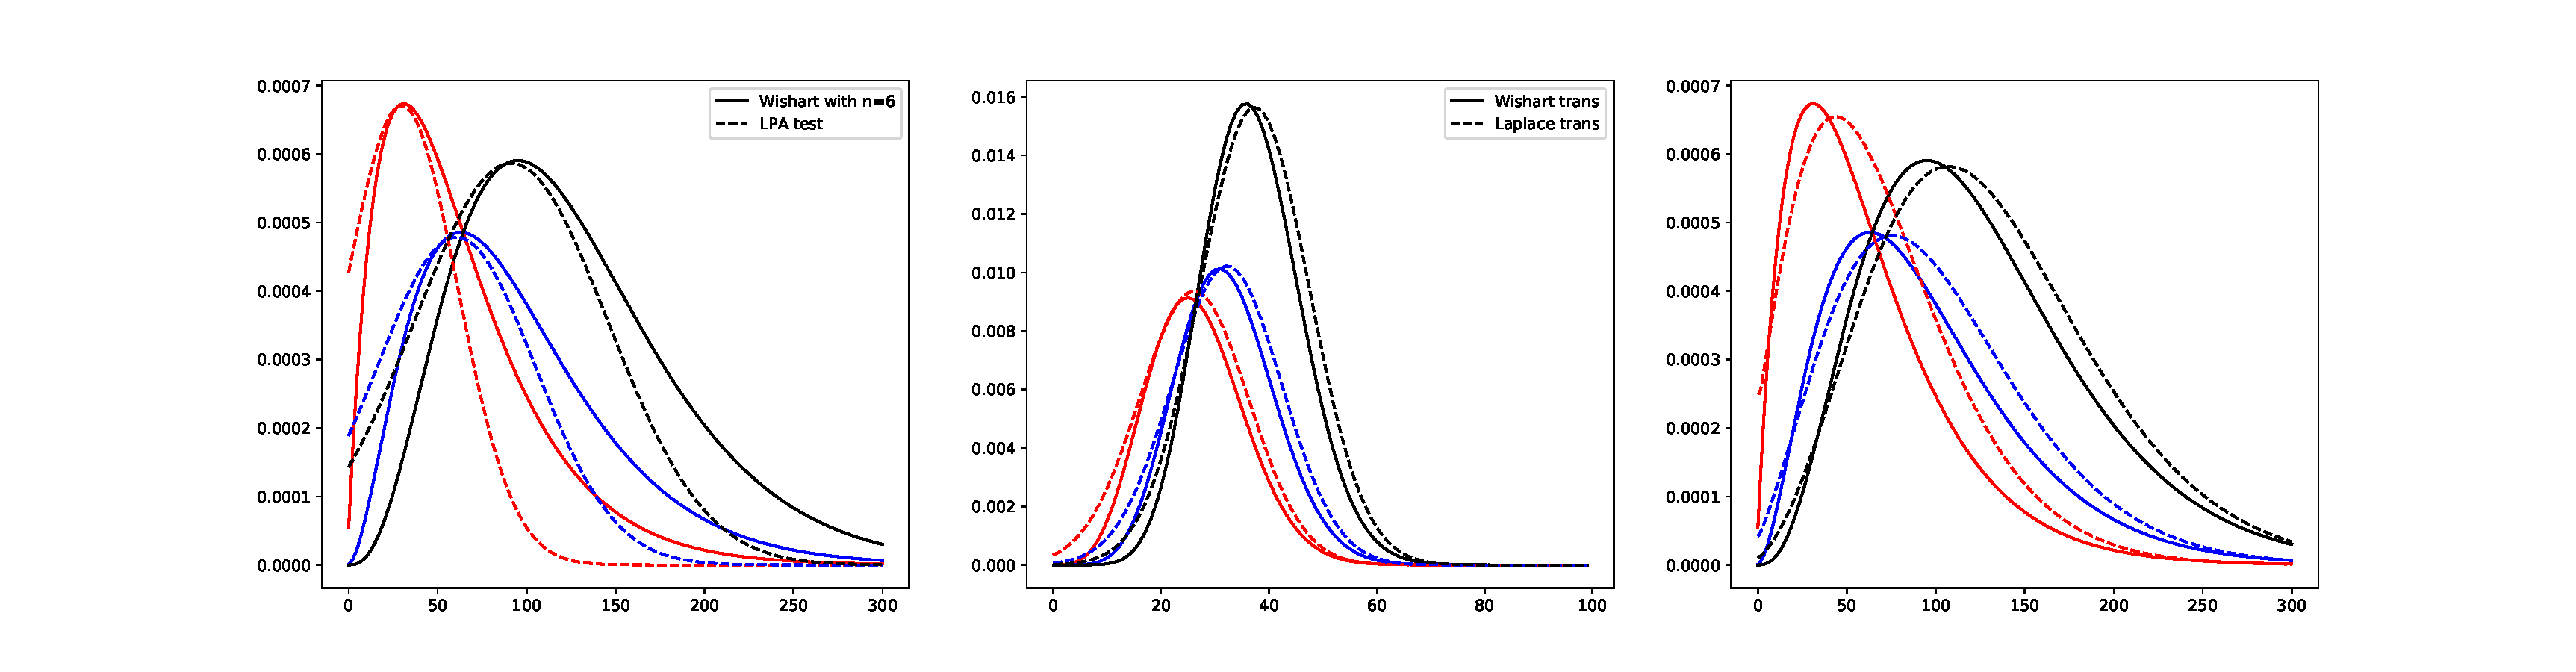
\includegraphics[width=\textwidth]{figures/wishart_playground_sqrtm.pdf}
	\caption{wishart comparison for sqrtm}
	\label{fig:wishart_comparison}
\end{figure}




\subsection{Standard Inverse Wishart distribution}

the pdf of the Inverse Wishart is

\begin{subequations}
\begin{align}
\mathcal{IW}_{\mathbf x}({\mathbf x}; {\mathbf \Psi}, \nu) &= \frac{\left|{\mathbf\Psi}\right|^{\nu/2}}{2^{\nu p/2}\Gamma_p(\frac \nu 2)} \left|\mathbf{x}\right|^{-(\nu+p+1)/2} e^{-\frac{1}{2}\operatorname{tr}(\mathbf\Psi\mathbf{x}^{-1})}
\label{eq:inverse_wishart_pdf} \\
&= \exp \left[-(\nu + p + 1)/2 \log(|x|) - \frac{1}{2} \text{tr}(\Psi x^{-1}) + \log(\frac{\left|{\mathbf\Psi}\right|^{\nu/2}}{2^{\nu p/2}\Gamma_p(\frac \nu 2)}) \right]
\end{align}
\end{subequations}

with $h(X) = 1/X^\frac{1}{2}, \phi(X)=(\log(X), X^{-1}), w=(-(\nu+p)/2, \Psi)$ and $Z(n,p,V)=- \log(\frac{\left|{\mathbf\Psi}\right|^{\nu/2}}{2^{\nu p/2}\Gamma_p(\frac \nu 2)})$.

\subsubsection{Laplace Approximation of the standard inverse Wishart distribution}

Using $\frac{\partial \det(X)}{\partial X} = \det(X)(X^{-1})^\top$ and $\frac{\partial}{\partial X} \operatorname{tr}(AX)^{-1} = (X^{-1}AX^{-1})^\top$ we can calculate the mode by setting the first derivative of the log-pdf to zero:

\begin{subequations}
\begin{align}
	\frac{\partial \log \mathcal{IW}_{\mathbf X}({\mathbf X}; {\mathbf \Psi}, \nu)}{\partial X} &= \frac{-(\nu + p + 1) \det(X) X^{-\top}}{2\det(X)} + \frac{(X^{-1} \Psi X^{-1})^\top}{2} \\
	&=\frac{-(\nu + p + 1) X^{-\top}}{2} + \frac{(X^{-1} \Psi X^{-1})^\top}{2} \\
	\Rightarrow 0 &=\frac{-(\nu + p + 1) X^{-\top}}{2} + \frac{(X^{-1} \Psi X^{-1})^\top}{2} \\
	\Leftrightarrow (\nu + p + 1) X^{-1} &= X^{-1} \Psi X^{-1} \\
	\Leftrightarrow (\nu + p + 1) &= X^{-1} \Psi\\
	\Leftrightarrow X &= \frac{1}{\nu + p + 1} \Psi
\end{align}
\end{subequations}

Using 

\begin{align}
	\frac{\partial(XBX)_{kl}}{\partial X_{ij}} &= \delta_{ki}(BX)_{lj} + \delta_{lj}(XB)_{ki} \\
	\frac{\partial X^{-1}}{\partial X} &= -(X^{-1} \otimes X^{-1}) \\
	\frac{\partial (X^{-1}B X^{-1})}{\partial X} &= \frac{\partial (X^{-1}B X^{-1})}{\partial X^{-1}} \frac{\partial X^{-1}}{\partial X} = -[\delta_{ki}(BX^{-1})_{lj} + \delta_{lj}(X^{-1}B)_{ki}] (X^{-1} \otimes X^{-1})\\
	(AB)^{-1} &= B^{-1} A^{-1}
\end{align}

we can get the covariance matrix by inverting the Hessian and multiplying with -1. 

\begin{subequations}
\begin{align}
		\frac{\partial^2 \log f_{\mathbf X}({\mathbf X}; {\mathbf \Psi}, \nu)}{\partial^2 X} &= \frac{(\nu + p + 1)}{2}(X^{-1} \otimes X^{-1})^\top - \frac{[\delta_{ki}(\Psi X^{-1})_{lj} + \delta_{lj}(X^{-1}\Psi)_{ki}]}{2} (X^{-1} \otimes X^{-1})^\top \\
		&= \left\{\frac{(\nu + p + 1)}{2} I_{n^2}- \frac{[\delta_{ki}(\Psi X^{-1})_{lj} + \delta_{lj}(X^{-1}\Psi)_{ki}]}{2}\right\} (X^{-1} \otimes X^{-1})^\top \\
		&\overset{\text{insert mode}}{=} \left\{\frac{(\nu + p + 1)}{2} I_{n^2}- \frac{[\delta_{ki}((\nu + p + 1)\Psi \Psi^{-1})_{lj} + \delta_{lj}((\nu + p + 1)\Psi^{-1}\Psi)_{ki}]}{2}\right\} (\nu + p + 1)^2(\psi \otimes \psi)^{-\top} \\
		&= \left\{\frac{(\nu + p + 1)}{2} I_{n^2}- \underbrace{\frac{[\delta_{ki}((\nu + p + 1)I_n)_{lj} + \delta_{lj}((\nu + p + 1)I_n)_{ki}]}{2}}_{=(\nu + p + 1)I_{n^2}}\right\} (\nu + p + 1)^2(\psi \otimes \psi)^{-\top} \\
		&= -\underbrace{\frac{1}{2}(\nu + p + 1) I_{n^2}}_{A} \underbrace{(\nu + p + 1)^2(\psi \otimes \psi)^{-\top}}_{B} \\
		&\overset{\text{invert}}{\Rightarrow} -\frac{1}{(\nu + p + 1)^2}(\psi \otimes \psi)^{\top} \frac{2}{(\nu + p + 1)}I_{n^2} \\
		&=\overset{\cdot -1}{\Rightarrow} \Sigma = \frac{2}{(\nu + p + 1)^3}(\Psi \otimes \Psi)^\top
\end{align}
\end{subequations}

where $I_{n}$ and $I_n^2$ are the identity matrix of size $n$ and $n^2$ respectively. We can also ignore the transpose since we are dealing with symmetric positive definite matrices when it comes to the inverse Wishart distribution. This yields a multivariate Normal of the form $\mathcal{N}\left(X; \mu = \frac{1}{\nu + p + 1} \Psi, \Sigma = \frac{2}{(\nu + p + 1)^3}(\Psi \otimes \Psi)^\top\right)$. 

\subsection{Logm-Transformed inverse Wishart distribution}

we transform the distribution with $g(X) = \text{logm}(X)$, i.e. $X(Y) = g^{-1}(X) = \text{expm}(Y)$, where $\operatorname{expm}(Y)$ is the matrix exponential. The new pdf becomes 

\begin{subequations}
\begin{align}
	\mathcal{IW}_{logm}({\mathbf Y}; {\mathbf \Psi}, \nu) &= \frac{\left|{\mathbf\Psi}\right|^{\nu/2}}{2^{\nu p/2}\Gamma_p(\frac \nu 2)} \left|\operatorname{expm}\mathbf{Y}\right|^{-(\nu+p+1)/2} e^{-\frac{1}{2}\operatorname{tr}(\mathbf\Psi(\operatorname{expm}\mathbf{Y})^{-1})} \cdot |\operatorname{expm}(\mathbf{Y})|\\
	&=  \frac{\left|{\mathbf\Psi}\right|^{\nu/2}}{2^{\nu p/2}\Gamma_p(\frac \nu 2)} \left|\operatorname{expm}\mathbf{Y}\right|^{-(\nu+p-1)/2} e^{-\frac{1}{2}\operatorname{tr}(\mathbf\Psi(\operatorname{expm}\mathbf{Y})^{-1})} \\
	&= \exp\left[C - (\nu+p-1)/2\log  \left|\operatorname{expm}\mathbf{Y}\right| - -\frac{1}{2}\operatorname{tr}(\mathbf\Psi\operatorname{expm}(\mathbf{-Y}))\right]
\end{align}
\end{subequations}

with exponential family statistics $h(Y) = Y^\frac{1}{2}, \phi(Y) = (\log(\det(\operatorname{expm}(Y))), \operatorname{expm}(Y)), w = ((\nu + p)/2, \Psi)$ and $Z(n,p,V)=- \log\left(\frac{\left|{\mathbf\Psi}\right|^{\nu/2}}{2^{\nu p/2}\Gamma_p(\frac \nu 2)}\right)$

\subsubsection{Laplace Approximation of the logm-transformed inverse Wishart distribution}

For the first derivative we use the same ideas as for the Wishart (TODO:link). 

\begin{subequations}
\begin{align}
	\frac{\partial \log \mathcal{IW}_{logm}}{\partial Y} &= \frac{\partial}{\partial Y} -(\nu+p-1)/2\log  \left|\operatorname{expm}\mathbf{Y}\right| - -\frac{1}{2}\operatorname{tr}(\mathbf\Psi\operatorname{expm}(\mathbf{-Y}))\\
	&= -\frac{(\nu+p-1)}{2} + \frac{1}{2}\mathbf\Psi\operatorname{expm}(\mathbf{-Y})
\end{align}
\end{subequations}

which yields the mode by setting it to zero and solving for $Y$.

\begin{subequations}
\begin{align}
	0 &= -\frac{(\nu+p-1)}{2} + \frac{1}{2}\mathbf\Psi\operatorname{expm}(\mathbf{-Y}) \\
	\Leftrightarrow (\nu+p-1) I_p &=  \mathbf\Psi(\operatorname{expm}(\mathbf{Y}))^{-1} \\
	\Leftrightarrow Y &= \operatorname{logm}\left(\frac{\mathbf\Psi}{n+p-1}\right)
\end{align}
\end{subequations}

For the second derivative we also use the same ideas as for the Wishart (TODO: link + rewrite). 

\begin{subequations}
\begin{align}
	\frac{\partial^2 \log \mathcal{IW}_{logm}}{\partial^2 Y} &= \frac{\partial }{\partial Y} \left[-\frac{(\nu+p-1)}{2} + \frac{1}{2}\mathbf\Psi\operatorname{expm}(\mathbf{-Y}) \right] \\
	&= -\frac{1}{2}\left[\mathbf\Psi\operatorname{expm}(\mathbf{Y})^{-1} \otimes I_p\right] \\
	&\overset{\text{mode}}{\Rightarrow} -\frac{1}{2}\left[\mathbf\Psi\frac{\mathbf\Psi^{-1}}{(\nu+p-1)} \otimes I_p\right] \\
	&= -\frac{1}{2(\nu+p-1)} I_{p\times p} \\
	\Rightarrow \Sigma &= 2(\nu+p-1) I_{p\times p}
\end{align}
\end{subequations}

This yields a multivariate Normal distribution $\mathcal{N}\left(Y; \mu = \operatorname{logm}\left(\frac{\mathbf\Psi}{n+p-1}\right), \Sigma = 2(\nu+p-1) I_{p\times p}\right)$. 

\subsubsection{The Bridge for the logm-transformed inverse Wishart distribution}

We get $\mu$ and $\Psi$ from the Laplace approximation and determine $V$ by inverting $\mu$

\begin{subequations}
\begin{align}
	\mu = \operatorname{logm}\left(\frac{\mathbf\Psi}{n+p-1}\right) \Leftrightarrow \operatorname{expm}(\mu) = \frac{\mathbf\Psi}{n+p-1} \Leftrightarrow \mathbf\Psi = \operatorname{expm}(\mu)(n+p-1)
\end{align}
\end{subequations}

In summary: 

\begin{subequations}
\begin{align}
	\mu &= \operatorname{logm}\left(\frac{\mathbf\Psi}{n+p-1}\right) \\
	\Sigma &= 2(\nu+p-1) I_{p\times p} \\
	\mathbf{\Psi} &=  (\nu+p-1)\operatorname{expm}(\mu) \\
	\nu &= ?
\end{align}
\end{subequations}

where $\mathbf{\Psi}$ is reshaped to a $p \times p$ matrix. 

\subsection{Sqrtm-Transformed inverse Wishart distribution}

we transform the distribution with $g(X) = \text{sqrtm}(X) = X^{\frac{1}{2}}$, i.e. $X(Y) = g^{-1}(X) = Y^2$, where $\text{sqrtm}(Y)$ is the square root of the matrix. The new pdf becomes 

\begin{subequations}
\begin{align}
	\mathcal{IW}_{\operatorname{sqrtm}}({\mathbf Y}; {\mathbf \Psi}, \nu) &= \frac{\left|{\mathbf\Psi}\right|^{\nu/2}}{2^{\nu p/2}\Gamma_p(\frac \nu 2)} \left|\mathbf{Y^2}\right|^{-(\nu+p+1)/2} e^{-\frac{1}{2}\operatorname{tr}(\mathbf\Psi\mathbf{Y}^{-2})} |2Y| \\
	&= \frac{\left|{\mathbf\Psi}\right|^{\nu/2}}{2^{\nu p/2}\Gamma_p(\frac \nu 2)} \left|\mathbf{Y}\right|^{-(\nu+p+1)} e^{-\frac{1}{2}\operatorname{tr}(\mathbf\Psi\mathbf{Y}^{-2})} 2^p|Y| \\
	&= \frac{\left|{\mathbf\Psi}\right|^{\nu/2}}{2^{\nu p/2}\Gamma_p(\frac \nu 2)} \left|\mathbf{Y}\right|^{-(\nu+p)} e^{-\frac{1}{2}\operatorname{tr}(\mathbf\Psi\mathbf{Y}^{-2})} 2^p \\ 
	&= \exp\left[-(\nu + p) \log(|Y|) - \frac{1}{2}\text{tr}(\Psi Y^{-2}) + \log(C)\right]
\end{align}
\end{subequations}

with $h(Y) = 1, \phi(Y) = (\log(|Y|), Y^{-2}), w = (-(\nu + p), \Psi)$ and $Z(w) = \log\left( \frac{\left|{\mathbf\Psi}\right|^{\nu/2}}{2^{\nu p/2}\Gamma_p(\frac \nu 2)}\right)$. 

\subsubsection{Laplace Approximation of the sqrtm-transformed inverse Wishart distribution}

Using 

\begin{align}
	\frac{\partial \operatorname{tr}(\Psi Y^{-2})}{\partial Y} &= \frac{1}{2}[Y^{-1}\Psi Y^{-2} + Y^{-2}\Psi Y^{-1}]^\top 
\end{align}

we can calculate the mode by setting the derivative of the log-pdf to zero:

\begin{subequations}
\begin{align}
	\frac{\partial \log \mathcal{IW}_{\text{sqrtm}}(Y, \Psi, \nu)}{\partial Y} &= \frac{-(\nu + p )\det(Y) Y^{-\top}}{\det(Y)} + \frac{1}{2}[Y^{-1}\Psi Y^{-2} + Y^{-2}\Psi Y^{-1}]^\top \\
	&= -(\nu + p)Y^{-\top} + \frac{1}{2}[Y^{-1}\Psi Y^{-2} + Y^{-2}\Psi Y^{-1}]^\top \\
	\Rightarrow (\nu + p)Y^{-1} &= \frac{1}{2}[Y^{-1}\Psi Y^{-2} + Y^{-2}\Psi Y^{-1}] \\
	\Rightarrow 2(\nu + p)I_p &= [Y^{-1}\Psi Y^{-1} + Y^{-2}\Psi] \\
	\Leftrightarrow Y = ?
\end{align}
\end{subequations}

Using

\begin{align}
	\frac{\partial(XVXX)_{kl}}{\partial X_{ij}} &= \frac{\partial}{\partial X_{ij}} \sum_{u_1, u_2, u_3} X_{k,u_1} V_{u_1, u_2} X_{u_2, u_3} X_{u_3, l} \\
	&= \delta_{i,k} \delta_{j,u_1} V_{u_1, u_2} X_{u_2, u_3} X_{u_3, l} \\
	&+ X_{k,u_1} V_{u_1, u_2} \delta_{i,u_2} \delta_{j,u_3}X_{u_3, l} \\
	&+ X_{k,u_1} V_{u_1, u_2} X_{u_2, u_3}\delta_{i,u_3} \delta_{j,l} \\
	&= I_{k,i} \cdot (VXX)_{j,l} + (XV)_{k,i} \cdot (X)_{j,l} + (XVX)_{k,i} \cdot I_{j,l} \\
	\Rightarrow \frac{\partial XVXX}{\partial X} &=  I \otimes VXX + XV \otimes X + XVX \otimes I \\
	\frac{\partial (X^{-1} V X^{-1} X^{-1})^\top}{\partial X} &= -[I \boxtimes VX^{-1}X^{-1} + (X^{-1}V)^\top \boxtimes X^{-1} + (X^{-1}VX^{-1})^\top \boxtimes I]^T (X^{-1} \boxtimes X^{-\top}) \\
	\frac{\partial (X^{-1} X^{-1} V X^{-1})^\top}{\partial X} &= -[I \boxtimes X^{-1}VX^{-1} + X^{-^\top} \boxtimes VX^{-1} + (X^{-1}X^{-1}V)^\top \boxtimes I]^T (X^{-1} \boxtimes X^{-\top})
\end{align}

With these rules we can calculate the Hessian

\begin{subequations}
\begin{align}
	\frac{\partial^2 \log \mathcal{IW}_{\text{sqrtm}}(Y, \Psi, \nu)}{\partial^2 Y} &= \frac{\partial}{\partial Y} -(\nu + p)Y^{-\top} + \frac{1}{2}[Y^{-1}\Psi Y^{-2} + Y^{-2}\Psi Y^{-1}]^\top \\ 
	&\overset{\text{symmetry}}{=}\frac{\partial}{\partial Y} -(\nu + p)Y^{-1} + \frac{1}{2}[Y^{-1}\Psi Y^{-2} + Y^{-2}\Psi Y^{-1}]^\top \\
	&= (\nu + p)(Y^{-1} \otimes Y^{-\top}) \\
	&- \frac{1}{2}\{[I \boxtimes \Psi Y^{-1}Y^{-1} + (Y^{-1}\Psi)^\top \boxtimes Y^{-1} + (Y^{-1}\Psi Y^{-1})^\top \boxtimes I]^T (Y^{-1} \boxtimes Y^{-\top}) \\
	&+ [I \boxtimes Y^{-1}\Psi Y^{-1} + Y^{-^\top} \boxtimes \Psi Y^{-1} + (Y^{-1}Y^{-1}\Psi)^\top \boxtimes I]^T (Y^{-1} \boxtimes Y^{-\top})\} \\
\end{align}
\end{subequations}

However, since we don't know the solution to the mode this result is of limited value to us. 

However, if we choose the the approximation 
\begin{align}
\frac{\partial \operatorname{tr}(\Psi Y^{-2})}{\partial Y} &= \frac{1}{2}[Y^{-1}\Psi Y^{-2} + Y^{-2}\Psi Y^{-1}]^\top \approx 2\Psi X^{-3}
\end{align}
we can find explicit formulations of the mode and covariance matrix. The mode is

\begin{subequations}
\begin{align}
\frac{\partial \log \mathcal{IW}'_{\text{sqrtm}}(Y, \Psi, \nu)}{\partial Y} &= \frac{-(\nu + p )\det(Y) Y^{-\top}}{\det(Y)} + \frac{1}{2} 2 \Psi Y^{-3}
&= -(\nu + p)Y^{-\top} + \Psi Y^{-3} \\
\Rightarrow (\nu + p)Y^{-1} &= \Psi Y^{-3} \\
\Leftrightarrow (\nu + p)\Psi^{-1} &= Y^{-2} \\
\Leftrightarrow Y &= \operatorname{sqrtm}\left(\frac{1}{(\nu+p)} \Psi^{-1}\right)
\end{align}
\end{subequations}

It also means we can compute the Hessian and insert the mode

\begin{subequations}
\begin{align}
	\frac{\partial^2 \log \mathcal{IW}_{\text{sqrtm}}(Y, \Psi, \nu)}{\partial^2 Y} &= \frac{\partial}{\partial Y} -(\nu + p)Y^{-\top} + (\Psi Y^{-3})^\top \\ 
	&= \frac{\partial}{\partial Y} -(\nu + p)Y^{-\top} + (Y^{-\top}Y^{-\top}Y^{-\top}\Psi^\top Y^{-3}) \\
	&\overset{\text{symmetry}}{=}\frac{\partial}{\partial Y} -(\nu + p)Y^{-1} + Y^{-3} \Psi \\
	&= (\nu + p)(X^{-1} \otimes X^{-1}) - [I_p \otimes X^{-2}\Psi + X^{-1} \otimes X^{-1}\Psi + X^{-2} \otimes V](X^{-1} \otimes X^{-1}) \\
	&= (\nu + p)(X^{-1} \otimes X^{-1}) - [X^{-1} \otimes X^{-3}\Psi + X^{-2} \otimes X^{-2}V + X^{-3} \otimes VX^{-1}]\\
	&\overset{\text{mode}}{\Rightarrow} (\nu + p)^2 (\Psi^{-\frac{1}{2}} \otimes \Psi^{-\frac{1}{2}}) - (\nu+p)^2[\Psi^{-\frac{1}{2}} \otimes \Psi^{-\frac{1}{2}} + \Psi^{-1} \otimes I_p + \Psi^{-\frac{3}{2}} \otimes \Psi^{\frac{1}{2}}] \\
	&= - (\nu+p)^2[\Psi^{-1} \otimes I_p + \Psi^{-\frac{3}{2}} \otimes \Psi^{\frac{1}{2}}] \\
	&= - (\nu+p)^2[(\Psi^{-\frac{3}{2}} \otimes \Psi^{\frac{1}{2}})(\Psi^{\frac{1}{2}} \otimes \Psi^{\frac{1}{2}} + I_{p^2})] \\
	\Rightarrow \Sigma &= 1/(\nu+p)^2 [(\Psi^{-\frac{3}{2}} \otimes \Psi^{\frac{1}{2}})(\Psi^{\frac{1}{2}} \otimes \Psi^{\frac{1}{2}} + I_{p^2})]^{-1}
\end{align}
\end{subequations}

which could be inverted more easily using equation 5 of \url{http://papers.nips.cc/paper/4281-efficient-inference-in-matrix-variate-gaussian-models-with-iid-observation-noise.pdf}

\subsubsection{The Bridge for the sqrtm-transformed inverse Wishart distribution}

TODO
